% Options for packages loaded elsewhere
% Options for packages loaded elsewhere
\PassOptionsToPackage{unicode}{hyperref}
\PassOptionsToPackage{hyphens}{url}
\PassOptionsToPackage{dvipsnames,svgnames,x11names}{xcolor}
%
\documentclass[
  russian,
  letterpaper,
  DIV=11,
  numbers=noendperiod]{scrartcl}
\usepackage{xcolor}
\usepackage{amsmath,amssymb}
\setcounter{secnumdepth}{5}
\usepackage{iftex}
\ifPDFTeX
  \usepackage[T1]{fontenc}
  \usepackage[utf8]{inputenc}
  \usepackage{textcomp} % provide euro and other symbols
\else % if luatex or xetex
  \usepackage{unicode-math} % this also loads fontspec
  \defaultfontfeatures{Scale=MatchLowercase}
  \defaultfontfeatures[\rmfamily]{Ligatures=TeX,Scale=1}
\fi
\usepackage{lmodern}
\ifPDFTeX\else
  % xetex/luatex font selection
\fi
% Use upquote if available, for straight quotes in verbatim environments
\IfFileExists{upquote.sty}{\usepackage{upquote}}{}
\IfFileExists{microtype.sty}{% use microtype if available
  \usepackage[]{microtype}
  \UseMicrotypeSet[protrusion]{basicmath} % disable protrusion for tt fonts
}{}
\makeatletter
\@ifundefined{KOMAClassName}{% if non-KOMA class
  \IfFileExists{parskip.sty}{%
    \usepackage{parskip}
  }{% else
    \setlength{\parindent}{0pt}
    \setlength{\parskip}{6pt plus 2pt minus 1pt}}
}{% if KOMA class
  \KOMAoptions{parskip=half}}
\makeatother
% Make \paragraph and \subparagraph free-standing
\makeatletter
\ifx\paragraph\undefined\else
  \let\oldparagraph\paragraph
  \renewcommand{\paragraph}{
    \@ifstar
      \xxxParagraphStar
      \xxxParagraphNoStar
  }
  \newcommand{\xxxParagraphStar}[1]{\oldparagraph*{#1}\mbox{}}
  \newcommand{\xxxParagraphNoStar}[1]{\oldparagraph{#1}\mbox{}}
\fi
\ifx\subparagraph\undefined\else
  \let\oldsubparagraph\subparagraph
  \renewcommand{\subparagraph}{
    \@ifstar
      \xxxSubParagraphStar
      \xxxSubParagraphNoStar
  }
  \newcommand{\xxxSubParagraphStar}[1]{\oldsubparagraph*{#1}\mbox{}}
  \newcommand{\xxxSubParagraphNoStar}[1]{\oldsubparagraph{#1}\mbox{}}
\fi
\makeatother

\usepackage{color}
\usepackage{fancyvrb}
\newcommand{\VerbBar}{|}
\newcommand{\VERB}{\Verb[commandchars=\\\{\}]}
\DefineVerbatimEnvironment{Highlighting}{Verbatim}{commandchars=\\\{\}}
% Add ',fontsize=\small' for more characters per line
\usepackage{framed}
\definecolor{shadecolor}{RGB}{241,243,245}
\newenvironment{Shaded}{\begin{snugshade}}{\end{snugshade}}
\newcommand{\AlertTok}[1]{\textcolor[rgb]{0.68,0.00,0.00}{#1}}
\newcommand{\AnnotationTok}[1]{\textcolor[rgb]{0.37,0.37,0.37}{#1}}
\newcommand{\AttributeTok}[1]{\textcolor[rgb]{0.40,0.45,0.13}{#1}}
\newcommand{\BaseNTok}[1]{\textcolor[rgb]{0.68,0.00,0.00}{#1}}
\newcommand{\BuiltInTok}[1]{\textcolor[rgb]{0.00,0.23,0.31}{#1}}
\newcommand{\CharTok}[1]{\textcolor[rgb]{0.13,0.47,0.30}{#1}}
\newcommand{\CommentTok}[1]{\textcolor[rgb]{0.37,0.37,0.37}{#1}}
\newcommand{\CommentVarTok}[1]{\textcolor[rgb]{0.37,0.37,0.37}{\textit{#1}}}
\newcommand{\ConstantTok}[1]{\textcolor[rgb]{0.56,0.35,0.01}{#1}}
\newcommand{\ControlFlowTok}[1]{\textcolor[rgb]{0.00,0.23,0.31}{\textbf{#1}}}
\newcommand{\DataTypeTok}[1]{\textcolor[rgb]{0.68,0.00,0.00}{#1}}
\newcommand{\DecValTok}[1]{\textcolor[rgb]{0.68,0.00,0.00}{#1}}
\newcommand{\DocumentationTok}[1]{\textcolor[rgb]{0.37,0.37,0.37}{\textit{#1}}}
\newcommand{\ErrorTok}[1]{\textcolor[rgb]{0.68,0.00,0.00}{#1}}
\newcommand{\ExtensionTok}[1]{\textcolor[rgb]{0.00,0.23,0.31}{#1}}
\newcommand{\FloatTok}[1]{\textcolor[rgb]{0.68,0.00,0.00}{#1}}
\newcommand{\FunctionTok}[1]{\textcolor[rgb]{0.28,0.35,0.67}{#1}}
\newcommand{\ImportTok}[1]{\textcolor[rgb]{0.00,0.46,0.62}{#1}}
\newcommand{\InformationTok}[1]{\textcolor[rgb]{0.37,0.37,0.37}{#1}}
\newcommand{\KeywordTok}[1]{\textcolor[rgb]{0.00,0.23,0.31}{\textbf{#1}}}
\newcommand{\NormalTok}[1]{\textcolor[rgb]{0.00,0.23,0.31}{#1}}
\newcommand{\OperatorTok}[1]{\textcolor[rgb]{0.37,0.37,0.37}{#1}}
\newcommand{\OtherTok}[1]{\textcolor[rgb]{0.00,0.23,0.31}{#1}}
\newcommand{\PreprocessorTok}[1]{\textcolor[rgb]{0.68,0.00,0.00}{#1}}
\newcommand{\RegionMarkerTok}[1]{\textcolor[rgb]{0.00,0.23,0.31}{#1}}
\newcommand{\SpecialCharTok}[1]{\textcolor[rgb]{0.37,0.37,0.37}{#1}}
\newcommand{\SpecialStringTok}[1]{\textcolor[rgb]{0.13,0.47,0.30}{#1}}
\newcommand{\StringTok}[1]{\textcolor[rgb]{0.13,0.47,0.30}{#1}}
\newcommand{\VariableTok}[1]{\textcolor[rgb]{0.07,0.07,0.07}{#1}}
\newcommand{\VerbatimStringTok}[1]{\textcolor[rgb]{0.13,0.47,0.30}{#1}}
\newcommand{\WarningTok}[1]{\textcolor[rgb]{0.37,0.37,0.37}{\textit{#1}}}

\usepackage{longtable,booktabs,array}
\usepackage{calc} % for calculating minipage widths
% Correct order of tables after \paragraph or \subparagraph
\usepackage{etoolbox}
\makeatletter
\patchcmd\longtable{\par}{\if@noskipsec\mbox{}\fi\par}{}{}
\makeatother
% Allow footnotes in longtable head/foot
\IfFileExists{footnotehyper.sty}{\usepackage{footnotehyper}}{\usepackage{footnote}}
\makesavenoteenv{longtable}
\usepackage{graphicx}
\makeatletter
\newsavebox\pandoc@box
\newcommand*\pandocbounded[1]{% scales image to fit in text height/width
  \sbox\pandoc@box{#1}%
  \Gscale@div\@tempa{\textheight}{\dimexpr\ht\pandoc@box+\dp\pandoc@box\relax}%
  \Gscale@div\@tempb{\linewidth}{\wd\pandoc@box}%
  \ifdim\@tempb\p@<\@tempa\p@\let\@tempa\@tempb\fi% select the smaller of both
  \ifdim\@tempa\p@<\p@\scalebox{\@tempa}{\usebox\pandoc@box}%
  \else\usebox{\pandoc@box}%
  \fi%
}
% Set default figure placement to htbp
\def\fps@figure{htbp}
\makeatother



\ifLuaTeX
\usepackage[bidi=basic,provide=*]{babel}
\else
\usepackage[bidi=default,provide=*]{babel}
\fi
% get rid of language-specific shorthands (see #6817):
\let\LanguageShortHands\languageshorthands
\def\languageshorthands#1{}


\setlength{\emergencystretch}{3em} % prevent overfull lines

\providecommand{\tightlist}{%
  \setlength{\itemsep}{0pt}\setlength{\parskip}{0pt}}



 


\usepackage{fontspec}

\setsansfont{Palatino Linotype}[
    Path=../files/palatino/,
    Extension = .ttf,
    UprightFont=palatino-Roman,
    BoldFont=palatino-Bold,
    ItalicFont=palatino-Italic,
    BoldItalicFont=palatino-BoldItalic
]
\setmainfont{Palatino Linotype}[
    Path=../files/palatino/,
    Extension = .ttf,
    UprightFont=palatino-Roman,
    BoldFont=palatino-Bold,
    ItalicFont=palatino-Italic,
    BoldItalicFont=palatino-BoldItalic
]

\usepackage[textwidth=0.86\paperwidth, textheight=0.86\paperheight]{geometry}
\usepackage{fancyhdr}
\usepackage{hyperref}
\usepackage{fontawesome5}
\usepackage{graphicx}
\usepackage{amssymb}
\usepackage{amsmath}
\graphicspath{{../files/}}

\newcommand{\R}{\mathbb{R}}

% \pagenumbering{gobble}
\pagestyle{fancy}
\fancyhead{} % clear all header fields
\fancyhead[R]{\href{https://cu25.fmin.xyz}{\faGem[regular]} \hspace{0.04cm} \href{https://github.com/MerkulovDaniil/cu25}{\faGithub} \hspace{0.07cm} \href{https://t.me/fminxyz}{\faTelegram}}
\fancyhead[L]{\href{https://fmin.xyz}{
\includegraphics[height=0.35cm]{logo.pdf}} \hspace{2pt} \textbf{Оптимизация для всех! ЦУ. 2025}}
\KOMAoption{captions}{tableheading}
\makeatletter
\@ifpackageloaded{tcolorbox}{}{\usepackage[skins,breakable]{tcolorbox}}
\@ifpackageloaded{fontawesome5}{}{\usepackage{fontawesome5}}
\definecolor{quarto-callout-color}{HTML}{909090}
\definecolor{quarto-callout-note-color}{HTML}{0758E5}
\definecolor{quarto-callout-important-color}{HTML}{CC1914}
\definecolor{quarto-callout-warning-color}{HTML}{EB9113}
\definecolor{quarto-callout-tip-color}{HTML}{00A047}
\definecolor{quarto-callout-caution-color}{HTML}{FC5300}
\definecolor{quarto-callout-color-frame}{HTML}{acacac}
\definecolor{quarto-callout-note-color-frame}{HTML}{4582ec}
\definecolor{quarto-callout-important-color-frame}{HTML}{d9534f}
\definecolor{quarto-callout-warning-color-frame}{HTML}{f0ad4e}
\definecolor{quarto-callout-tip-color-frame}{HTML}{02b875}
\definecolor{quarto-callout-caution-color-frame}{HTML}{fd7e14}
\makeatother
\makeatletter
\@ifpackageloaded{caption}{}{\usepackage{caption}}
\AtBeginDocument{%
\ifdefined\contentsname
  \renewcommand*\contentsname{Содержание}
\else
  \newcommand\contentsname{Содержание}
\fi
\ifdefined\listfigurename
  \renewcommand*\listfigurename{Список Иллюстраций}
\else
  \newcommand\listfigurename{Список Иллюстраций}
\fi
\ifdefined\listtablename
  \renewcommand*\listtablename{Список Таблиц}
\else
  \newcommand\listtablename{Список Таблиц}
\fi
\ifdefined\figurename
  \renewcommand*\figurename{Рисунок}
\else
  \newcommand\figurename{Рисунок}
\fi
\ifdefined\tablename
  \renewcommand*\tablename{Таблица}
\else
  \newcommand\tablename{Таблица}
\fi
}
\@ifpackageloaded{float}{}{\usepackage{float}}
\floatstyle{ruled}
\@ifundefined{c@chapter}{\newfloat{codelisting}{h}{lop}}{\newfloat{codelisting}{h}{lop}[chapter]}
\floatname{codelisting}{Список}
\newcommand*\listoflistings{\listof{codelisting}{Список Каталогов}}
\makeatother
\makeatletter
\makeatother
\makeatletter
\@ifpackageloaded{caption}{}{\usepackage{caption}}
\@ifpackageloaded{subcaption}{}{\usepackage{subcaption}}
\makeatother
\usepackage{bookmark}
\IfFileExists{xurl.sty}{\usepackage{xurl}}{} % add URL line breaks if available
\urlstyle{same}
\hypersetup{
  pdftitle={Матрично-векторное дифференцирование. Линейный поиск},
  pdfauthor={Даня Меркулов},
  pdflang={ru},
  colorlinks=true,
  linkcolor={blue},
  filecolor={Maroon},
  citecolor={Blue},
  urlcolor={Blue},
  pdfcreator={LaTeX via pandoc}}


\title{Матрично-векторное дифференцирование. Линейный поиск}
\author{Даня Меркулов}
\date{}
\begin{document}
\maketitle


\section{Матрично-векторное
дифференцирование}\label{ux43cux430ux442ux440ux438ux447ux43dux43e-ux432ux435ux43aux442ux43eux440ux43dux43eux435-ux434ux438ux444ux444ux435ux440ux435ux43dux446ux438ux440ux43eux432ux430ux43dux438ux435}

\subsection{Градиент}\label{ux433ux440ux430ux434ux438ux435ux43dux442}

Пусть \(f(x):\mathbb{R}^n\to\mathbb{R}\), тогда вектор, который содержит
все первые частные производные:

\[
\nabla f(x) = \dfrac{df}{dx} = \begin{pmatrix}
    \frac{\partial f}{\partial x_1} \\
    \frac{\partial f}{\partial x_2} \\
 \vdots \\
    \frac{\partial f}{\partial x_n}
\end{pmatrix}
\]

называется градиентом функции \(f(x)\). Этот вектор указывает
направление наискорейшего возрастания. Таким образом, вектор
\(-\nabla f(x)\) указывает направление наискорейшего убывания функции в
точке. Кроме того, вектор градиента всегда ортогонален линии уровня в
точке.

\begin{tcolorbox}[enhanced jigsaw, title=\textcolor{quarto-callout-color}{\faInfo}\hspace{0.5em}{Example}, colframe=quarto-callout-color-frame, colbacktitle=quarto-callout-color!10!white, arc=.35mm, left=2mm, toprule=.15mm, toptitle=1mm, opacitybacktitle=0.6, bottomtitle=1mm, leftrule=.75mm, breakable, colback=white, titlerule=0mm, opacityback=0, rightrule=.15mm, bottomrule=.15mm, coltitle=black]

Для функции \(f(x, y) = x^2 + y^2\) градиент равен: \[
\nabla f(x, y) =
\begin{bmatrix}
2x \\
2y \\
\end{bmatrix}
\] Он указывает направление наискорейшего возрастания функции.

\end{tcolorbox}

\begin{tcolorbox}[enhanced jigsaw, title=\textcolor{quarto-callout-color}{\faInfo}\hspace{0.5em}{Question}, colframe=quarto-callout-color-frame, colbacktitle=quarto-callout-color!10!white, arc=.35mm, left=2mm, toprule=.15mm, toptitle=1mm, opacitybacktitle=0.6, bottomtitle=1mm, leftrule=.75mm, breakable, colback=white, titlerule=0mm, opacityback=0, rightrule=.15mm, bottomrule=.15mm, coltitle=black]

Как связана норма градиента с крутизной функции?

\end{tcolorbox}

\subsection{Гессиан}\label{ux433ux435ux441ux441ux438ux430ux43d}

Пусть \(f(x):\mathbb{R}^n\to\mathbb{R}\), тогда матрица, содержащая все
вторые частные производные:

\[
f''(x) = \nabla^2 f(x) = \dfrac{\partial^2 f}{\partial x_i \partial x_j} = \begin{pmatrix}
    \frac{\partial^2 f}{\partial x_1 \partial x_1} & \frac{\partial^2 f}{\partial x_1 \partial x_2} & \dots  & \frac{\partial^2 f}{\partial x_1\partial x_n} \\
    \frac{\partial^2 f}{\partial x_2 \partial x_1} & \frac{\partial^2 f}{\partial x_2 \partial x_2} & \dots  & \frac{\partial^2 f}{\partial x_2 \partial x_n} \\
 \vdots & \vdots & \ddots & \vdots \\
    \frac{\partial^2 f}{\partial x_n \partial x_1} & \frac{\partial^2 f}{\partial x_n \partial x_2} & \dots  & \frac{\partial^2 f}{\partial x_n \partial x_n}
\end{pmatrix}
\]

Гессиан может быть тензором:
\(\left(f(x): \mathbb{R}^n \to \mathbb{R}^m \right)\) Таким образом, это
просто трехмерный тензор, каждый срез которого это гессиан
соответствующей скалярной функции
\(\left( \nabla^2f_1(x), \ldots, \nabla^2f_m(x)\right)\).

\begin{tcolorbox}[enhanced jigsaw, title=\textcolor{quarto-callout-color}{\faInfo}\hspace{0.5em}{Example}, colframe=quarto-callout-color-frame, colbacktitle=quarto-callout-color!10!white, arc=.35mm, left=2mm, toprule=.15mm, toptitle=1mm, opacitybacktitle=0.6, bottomtitle=1mm, leftrule=.75mm, breakable, colback=white, titlerule=0mm, opacityback=0, rightrule=.15mm, bottomrule=.15mm, coltitle=black]

Для функции \(f(x, y) = x^2 + y^2\) гессиан равен:

\[
H_f(x, y) = \begin{bmatrix} 2 & 0 \\
0 & 2 \\
\end{bmatrix}
\]

\end{tcolorbox}

Эта матрица содержит информацию о кривизне функции в разных
направлениях.

\begin{tcolorbox}[enhanced jigsaw, title=\textcolor{quarto-callout-color}{\faInfo}\hspace{0.5em}{Question}, colframe=quarto-callout-color-frame, colbacktitle=quarto-callout-color!10!white, arc=.35mm, left=2mm, toprule=.15mm, toptitle=1mm, opacitybacktitle=0.6, bottomtitle=1mm, leftrule=.75mm, breakable, colback=white, titlerule=0mm, opacityback=0, rightrule=.15mm, bottomrule=.15mm, coltitle=black]

Как можно использовать гессиан для определения выпуклости или вогнутости
функции?

\end{tcolorbox}

\subsection{Теорема
Шварца}\label{ux442ux435ux43eux440ux435ux43cux430-ux448ux432ux430ux440ux446ux430}

Пусть \(f: \mathbb{R}^n \rightarrow \mathbb{R}\) - функция. Если
смешанные частные производные
\(\frac{\partial^2 f}{\partial x_i \partial x_j}\) и
\(\frac{\partial^2 f}{\partial x_j \partial x_i}\) непрерывны на
открытом множестве, содержащем точку \(a\), то они равны в точке \(a\).
То есть, \[
\frac{\partial^2 f}{\partial x_i \partial x_j} (a) = \frac{\partial^2 f}{\partial x_j \partial x_i} (a)
\]

Согласно данной теореме, если смешанные частные производные непрерывны
на открытом множестве, то гессиан симметричен. То есть,

\[
\frac{\partial^2 f}{\partial x_i \partial x_j} = \frac{\partial^2 f}{\partial x_j \partial x_i} \quad \nabla^2 f(x)  =(\nabla^2 f(x))^T
\]

Эта симметричность упрощает вычисления и анализ, связанные с гессианом в
различных приложениях, особенно в оптимизации.

\begin{tcolorbox}[enhanced jigsaw, title=\textcolor{quarto-callout-color}{\faInfo}\hspace{0.5em}{Контрпример Шварца}, colframe=quarto-callout-color-frame, colbacktitle=quarto-callout-color!10!white, arc=.35mm, left=2mm, toprule=.15mm, toptitle=1mm, opacitybacktitle=0.6, bottomtitle=1mm, leftrule=.75mm, breakable, colback=white, titlerule=0mm, opacityback=0, rightrule=.15mm, bottomrule=.15mm, coltitle=black]

\[
f(x,y) = 
\begin{cases}
    \frac{xy\left(x^2 - y^2\right)}{x^2 + y^2} & \text{ для } (x,\, y) \ne (0,\, 0),\\
    0 & \text{ для } (x, y) = (0, 0).
\end{cases}
\] \pandocbounded{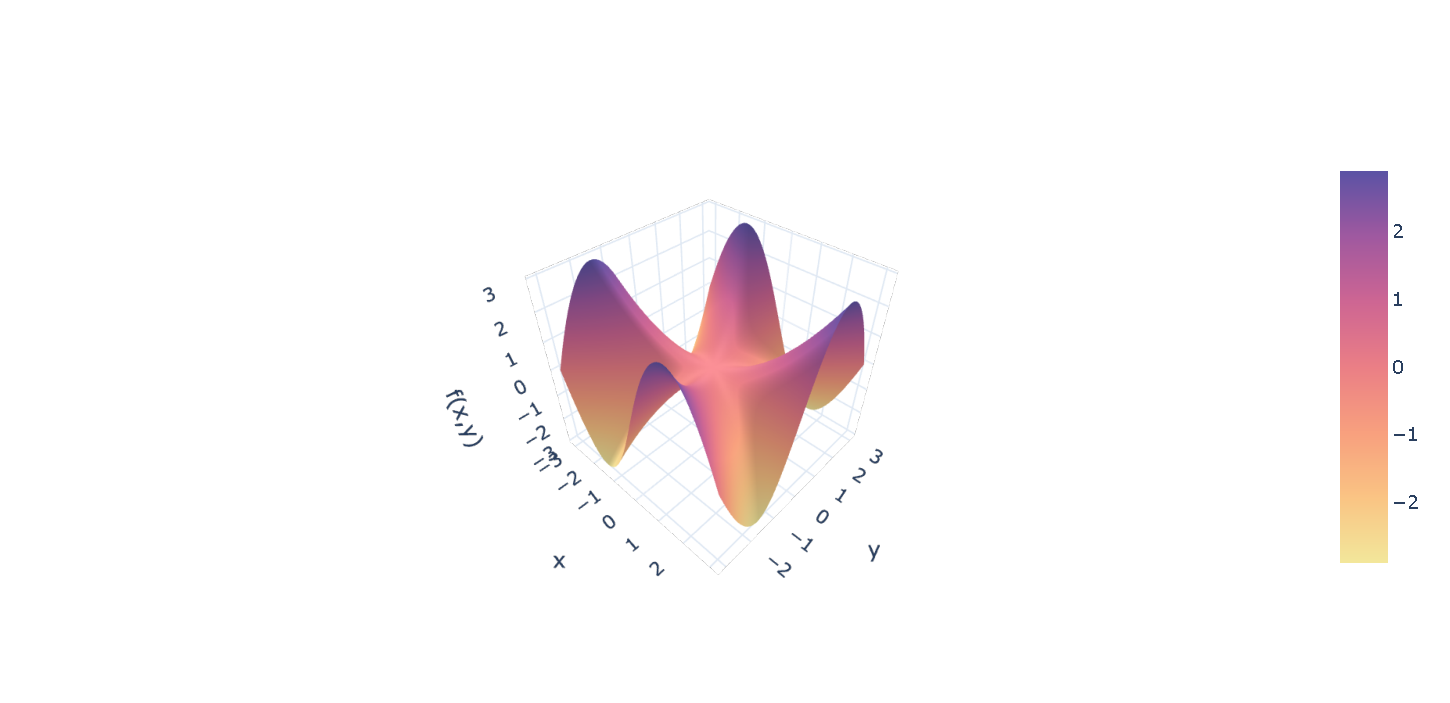
\includegraphics[keepaspectratio]{schwartz.pdf}} Можно
проверить, что
\(\frac{\partial^2 f}{ \partial x \partial y} (0, 0) \neq \frac{\partial^2 f}{ \partial y \partial x} (0, 0)\),
хотя смешанные частные производные существуют, и в каждой другой точке
симметричность выполняется.

\end{tcolorbox}

\subsection{Якобиан}\label{ux44fux43aux43eux431ux438ux430ux43d}

Обобщением понятия градиента на случай многомерной функции
\(f(x):\mathbb{R}^n\to\mathbb{R}^m\) является следующая матрица:

\[
J_f = f'(x) = \dfrac{df}{dx^T} = \begin{pmatrix}
    \frac{\partial f_1}{\partial x_1} & \frac{\partial f_2}{\partial x_1} & \dots  & \frac{\partial f_m}{\partial x_1} \\
    \frac{\partial f_1}{\partial x_2} & \frac{\partial f_2}{\partial x_2} & \dots  & \frac{\partial f_m}{\partial x_2} \\
 \vdots & \vdots & \ddots & \vdots \\
    \frac{\partial f_1}{\partial x_n} & \frac{\partial f_2}{\partial x_n} & \dots  & \frac{\partial f_m}{\partial x_n}
\end{pmatrix}
\]

Она содержит информацию о скорости изменения функции по отношению к ее
входу.

\begin{tcolorbox}[enhanced jigsaw, title=\textcolor{quarto-callout-color}{\faInfo}\hspace{0.5em}{Question}, colframe=quarto-callout-color-frame, colbacktitle=quarto-callout-color!10!white, arc=.35mm, left=2mm, toprule=.15mm, toptitle=1mm, opacitybacktitle=0.6, bottomtitle=1mm, leftrule=.75mm, breakable, colback=white, titlerule=0mm, opacityback=0, rightrule=.15mm, bottomrule=.15mm, coltitle=black]

Можно ли связать эти три определения выше (градиент, якобиан, и гессиан)
с помощью одного утверждения?

\end{tcolorbox}

\begin{tcolorbox}[enhanced jigsaw, title=\textcolor{quarto-callout-color}{\faInfo}\hspace{0.5em}{Example}, colframe=quarto-callout-color-frame, colbacktitle=quarto-callout-color!10!white, arc=.35mm, left=2mm, toprule=.15mm, toptitle=1mm, opacitybacktitle=0.6, bottomtitle=1mm, leftrule=.75mm, breakable, colback=white, titlerule=0mm, opacityback=0, rightrule=.15mm, bottomrule=.15mm, coltitle=black]

Для функции\\
\[
f(x, y) = \begin{bmatrix}
x + y \\
x - y \\
\end{bmatrix}, 
\] Якобиан равен: \[
J_f(x, y) = \begin{bmatrix}
1 & 1 \\
1 & -1 \\
\end{bmatrix}
\]

\end{tcolorbox}

\begin{tcolorbox}[enhanced jigsaw, title=\textcolor{quarto-callout-color}{\faInfo}\hspace{0.5em}{Question}, colframe=quarto-callout-color-frame, colbacktitle=quarto-callout-color!10!white, arc=.35mm, left=2mm, toprule=.15mm, toptitle=1mm, opacitybacktitle=0.6, bottomtitle=1mm, leftrule=.75mm, breakable, colback=white, titlerule=0mm, opacityback=0, rightrule=.15mm, bottomrule=.15mm, coltitle=black]

Как матрица Якоби связана с градиентом для скалярных функций?

\end{tcolorbox}

\subsection{Итог}\label{ux438ux442ux43eux433}

\[
f(x) : X \to Y; \qquad \frac{\partial f(x)}{\partial x} \in G
\]

\begin{longtable}[]{@{}
  >{\centering\arraybackslash}p{(\linewidth - 6\tabcolsep) * \real{0.2466}}
  >{\centering\arraybackslash}p{(\linewidth - 6\tabcolsep) * \real{0.2466}}
  >{\centering\arraybackslash}p{(\linewidth - 6\tabcolsep) * \real{0.2466}}
  >{\centering\arraybackslash}p{(\linewidth - 6\tabcolsep) * \real{0.2603}}@{}}
\toprule\noalign{}
\begin{minipage}[b]{\linewidth}\centering
X
\end{minipage} & \begin{minipage}[b]{\linewidth}\centering
Y
\end{minipage} & \begin{minipage}[b]{\linewidth}\centering
G
\end{minipage} & \begin{minipage}[b]{\linewidth}\centering
Name
\end{minipage} \\
\midrule\noalign{}
\endhead
\bottomrule\noalign{}
\endlastfoot
\(\mathbb{R}\) & \(\mathbb{R}\) & \(\mathbb{R}\) & \(f'(x)\)
(производная) \\
\(\mathbb{R}^n\) & \(\mathbb{R}\) & \(\mathbb{R}^n\) &
\(\dfrac{\partial f}{\partial x_i}\) (градиент) \\
\(\mathbb{R}^n\) & \(\mathbb{R}^m\) & \(\mathbb{R}^{n \times m}\) &
\(\dfrac{\partial f_i}{\partial x_j}\) (якобиан) \\
\(\mathbb{R}^{m \times n}\) & \(\mathbb{R}\) &
\(\mathbb{R}^{m \times n}\) & \(\dfrac{\partial f}{\partial x_{ij}}\) \\
\end{longtable}

\subsection{Аппроксимация Тейлора первого
порядка}\label{ux430ux43fux43fux440ux43eux43aux441ux438ux43cux430ux446ux438ux44f-ux442ux435ux439ux43bux43eux440ux430-ux43fux435ux440ux432ux43eux433ux43e-ux43fux43eux440ux44fux434ux43aux430}

Аппроксимация Тейлора первого порядка, также известная как линейное
приближение, строится вблизи некоторой точки \(x_0\). Если
\(f: \mathbb{R}^n \rightarrow \mathbb{R}\) - дифференцируемая функция,
то ее аппроксимация первого порядка задается следующим образом:

\[
f_{x_0}^I(x) = f(x_0) + \nabla f(x_0)^T (x - x_0)
\]

где:

\begin{itemize}
\tightlist
\item
  \(f(x_0)\) - значение функции в точке \(x_0\).
\item
  \(\nabla f(x_0)\) - градиент функции в точке \(x_0\).
\end{itemize}

Часто для упрощения теоретического анализа в некоторых методах заменяют
функцию вблизи некоторой точки на её аппроксимацию

\begin{figure}[H]

{\centering \pandocbounded{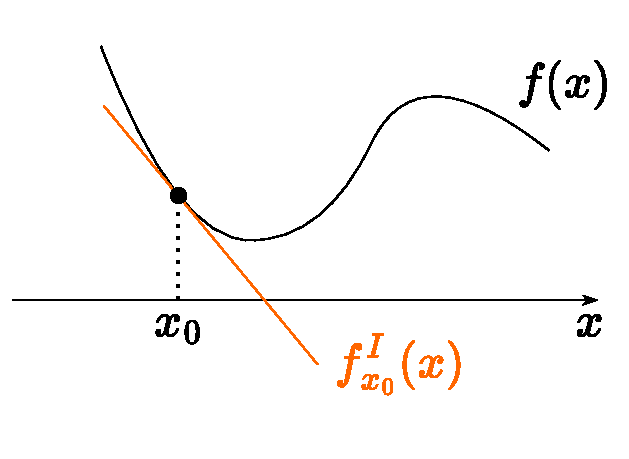
\includegraphics[keepaspectratio]{first_order_taylor.pdf}}

}

\caption{Аппроксимация Тейлора первого порядка в окрестности точки
\(x_0\)}

\end{figure}%

\subsection{Аппроксимация Тейлора второго
порядка}\label{ux430ux43fux43fux440ux43eux43aux441ux438ux43cux430ux446ux438ux44f-ux442ux435ux439ux43bux43eux440ux430-ux432ux442ux43eux440ux43eux433ux43e-ux43fux43eux440ux44fux434ux43aux430}

Аппроксимация Тейлора второго порядка, также известная как квадратичное
приближение, использует информацию о кривизне функции. Для дважды
дифференцируемой функции \(f: \mathbb{R}^n \rightarrow \mathbb{R}\), ее
аппроксимация второго порядка, строящаяся вблизи некоторой точки
\(x_0\), задается следующим образом:

\[
f_{x_0}^{II}(x) = f(x_0) + \nabla f(x_0)^T (x - x_0) + \frac{1}{2} (x - x_0)^T \nabla^2 f(x_0) (x - x_0)
\]

Где \(\nabla^2 f(x_0)\) - гессиан функции \(f\) в точке \(x_0\).

Когда линейного приближения функции не достаточно, можно рассмотреть
замену \(f(x)\) на \(f_{x_0}^{II}(x)\) в окрестности точки \(x_0\). В
общем, приближения Тейлора дают нам способ локально аппроксимировать
функции. Аппроксимация первого порядка определяется градиентом функции в
точке, т.е. нормалью к касательной гиперплоскости. А аппроксимация
второго порядка представляет из себя параболу Эти приближения особенно
полезны в оптимизации и численных методах, потому что они предоставляют
простой способ работы со сложными функциями.

\begin{figure}[H]

{\centering \pandocbounded{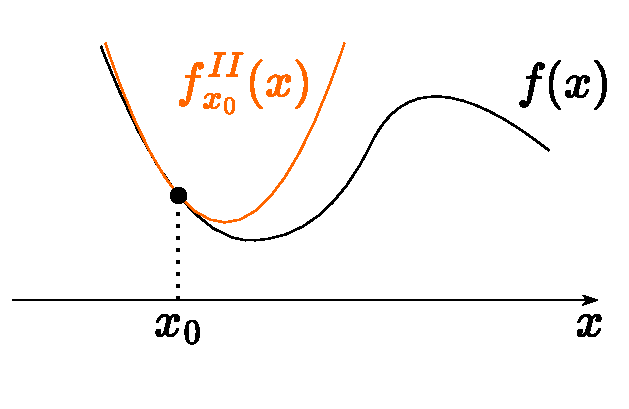
\includegraphics[keepaspectratio]{second_order_taylor.pdf}}

}

\caption{Аппроксимация Тейлора второго порядка в окрестности точки
\(x_0\)}

\end{figure}%

\section{Дифференциалы}\label{ux434ux438ux444ux444ux435ux440ux435ux43dux446ux438ux430ux43bux44b}

\begin{tcolorbox}[enhanced jigsaw, title=\textcolor{quarto-callout-color}{\faInfo}\hspace{0.5em}{Theorem}, colframe=quarto-callout-color-frame, colbacktitle=quarto-callout-color!10!white, arc=.35mm, left=2mm, toprule=.15mm, toptitle=1mm, opacitybacktitle=0.6, bottomtitle=1mm, leftrule=.75mm, breakable, colback=white, titlerule=0mm, opacityback=0, rightrule=.15mm, bottomrule=.15mm, coltitle=black]

Пусть \(x \in S\) - внутренняя точка множества \(S\), и пусть
\(D : U \rightarrow V\) - линейный оператор. Мы говорим, что функция
\(f\) дифференцируема в точке \(x\) с производной \(D\), если для всех
достаточно малых \(h \in U\) выполняется следующее разложение: \[ 
f(x + h) = f(x) + D[h] + o(\|h\|)
\] Если для любого линейного оператора \(D : U \rightarrow V\) функция
\(f\) не дифференцируема в точке \(x\) с производной \(D\), то мы
говорим, что \(f\) не дифференцируема в точке \(x\).

\end{tcolorbox}

После получения дифференциальной записи \(df\) мы можем получить
градиент, используя следующую формулу:

\[
df(x) = \langle \nabla f(x), dx\rangle
\]

Далее, если у нас есть дифференциал в такой форме и мы хотим вычислить
вторую производную матричной/векторной функции, мы рассматриваем
``старый'' \(dx\) как константу \(dx_1\), затем вычисляем
\(d(df) = d^2f(x)\)

\[
d^2f(x) = \langle \nabla^2 f(x) dx_1, dx\rangle = \langle H_f(x) dx_1, dx\rangle
\]

\subsection{Свойства
дифференциалов}\label{ux441ux432ux43eux439ux441ux442ux432ux430-ux434ux438ux444ux444ux435ux440ux435ux43dux446ux438ux430ux43bux43eux432}

Пусть \(A\) и \(B\) - постоянные матрицы, а \(X\) и \(Y\) - переменные
(или матричные функции).

\begin{itemize}
\tightlist
\item
  \(dA = 0\)
\item
  \(d(\alpha X) = \alpha (dX)\)
\item
  \(d(AXB) = A(dX )B\)
\item
  \(d(X+Y) = dX + dY\)
\item
  \(d(X^T) = (dX)^T\)
\item
  \(d(XY) = (dX)Y + X(dY)\)
\item
  \(d\langle X, Y\rangle = \langle dX, Y\rangle+ \langle X, dY\rangle\)
\end{itemize}

\begin{itemize}
\tightlist
\item
  \(d\left( \dfrac{X}{\phi}\right) = \dfrac{\phi dX - (d\phi) X}{\phi^2}\)
\item
  \(d\left( \det X \right) = \det X \langle X^{-T}, dX \rangle\)
\item
  \(d\left(\text{tr } X \right) = \langle I, dX\rangle\)
\item
  \(df(g(x)) = \dfrac{df}{dg} \cdot dg(x)\)
\item
  \(H = (J(\nabla f))^T\)
\item
  \(d(X^{-1})=-X^{-1}(dX)X^{-1}\)
\end{itemize}

\begin{tcolorbox}[enhanced jigsaw, title=\textcolor{quarto-callout-color}{\faInfo}\hspace{0.5em}{Example}, colframe=quarto-callout-color-frame, colbacktitle=quarto-callout-color!10!white, arc=.35mm, left=2mm, toprule=.15mm, toptitle=1mm, opacitybacktitle=0.6, bottomtitle=1mm, leftrule=.75mm, breakable, colback=white, titlerule=0mm, opacityback=0, rightrule=.15mm, bottomrule=.15mm, coltitle=black]

Найти \(df, \nabla f(x)\), если
\(f(x) = \langle x, Ax\rangle -b^T x + c\).

\end{tcolorbox}

\begin{tcolorbox}[enhanced jigsaw, title=\textcolor{quarto-callout-color}{\faInfo}\hspace{0.5em}{Example}, colframe=quarto-callout-color-frame, colbacktitle=quarto-callout-color!10!white, arc=.35mm, left=2mm, toprule=.15mm, toptitle=1mm, opacitybacktitle=0.6, bottomtitle=1mm, leftrule=.75mm, breakable, colback=white, titlerule=0mm, opacityback=0, rightrule=.15mm, bottomrule=.15mm, coltitle=black]

Найти \(df, \nabla f(x)\), если \(f(x) = \ln \langle x, Ax\rangle\).

\end{tcolorbox}

\begin{enumerate}
\def\labelenumi{\arabic{enumi}.}
\tightlist
\item
  Заметим, что \(A\) должна быть положительно определенной, потому что
  \(\langle x, Ax\rangle\) аргумент логарифма и для любого \(x\) формула
  должна быть положительной. Таким образом, \(A \in \mathbb{S}^n_{++}\)
  Давайте сначала найдем дифференциал: \[
  \begin{split}
   df &= d \left( \ln \langle x, Ax\rangle \right) = \dfrac{d \left( \langle x, Ax\rangle \right)}{ \langle x, Ax\rangle} = \dfrac{\langle dx, Ax\rangle +  \langle x, d(Ax)\rangle}{ \langle x, Ax\rangle} = \\
   &= \dfrac{\langle Ax, dx\rangle + \langle x, Adx\rangle}{ \langle x, Ax\rangle} = \dfrac{\langle Ax, dx\rangle + \langle A^T x, dx\rangle}{ \langle x, Ax\rangle} = \dfrac{\langle (A + A^T) x, dx\rangle}{ \langle x, Ax\rangle} 
  \end{split}
  \]
\item
  Наша основная цель - получить форму \(df = \langle \cdot, dx\rangle\)
  \[
  df = \left\langle  \dfrac{2 A x}{ \langle x, Ax\rangle} , dx\right\rangle
  \] Таким образом, градиент равен
  \(\nabla f(x) = \dfrac{2 A x}{ \langle x, Ax\rangle}\)
\end{enumerate}

\begin{tcolorbox}[enhanced jigsaw, title=\textcolor{quarto-callout-color}{\faInfo}\hspace{0.5em}{Example}, colframe=quarto-callout-color-frame, colbacktitle=quarto-callout-color!10!white, arc=.35mm, left=2mm, toprule=.15mm, toptitle=1mm, opacitybacktitle=0.6, bottomtitle=1mm, leftrule=.75mm, breakable, colback=white, titlerule=0mm, opacityback=0, rightrule=.15mm, bottomrule=.15mm, coltitle=black]

Найти \(df, \nabla f(X)\), если
\(f(X) = \langle S, X\rangle - \log \det X\).

\end{tcolorbox}

\section{Линейный
поиск}\label{ux43bux438ux43dux435ux439ux43dux44bux439-ux43fux43eux438ux441ux43a}

\subsection{Задача}\label{ux437ux430ux434ux430ux447ux430}

Предположим, у нас есть задача минимизации функции
\(f(x): \mathbb{R} \to \mathbb{R}\) скалярной переменной:

\[
f(x) \to \min_{x \in \mathbb{R}}
\]

Иногда мы рассматриваем похожую задачу поиска минимума функции на
отрезке \([a,b]\):

\[
f(x) \to \min_{x \in [a,b]}
\]

\begin{tcolorbox}[enhanced jigsaw, title=\textcolor{quarto-callout-color}{\faInfo}\hspace{0.5em}{Example}, colframe=quarto-callout-color-frame, colbacktitle=quarto-callout-color!10!white, arc=.35mm, left=2mm, toprule=.15mm, toptitle=1mm, opacitybacktitle=0.6, bottomtitle=1mm, leftrule=.75mm, breakable, colback=white, titlerule=0mm, opacityback=0, rightrule=.15mm, bottomrule=.15mm, coltitle=black]

Типичным примером задачи линейного поиска является выбор подходящего
шага для алгоритма градиентного спуска: \[
\begin{split}
x_{k+1} = x_k - \alpha \nabla f(x_k) \\
\alpha = \text{argmin } f(x_{k+1}) 
\end{split}
\]

\end{tcolorbox}

Линейный поиск является фундаментальной задачей оптимизации,
использующийся для решения сложных задач. Для упрощения предположим, что
\(f(x)\) \emph{унимодальна}, то есть имеет единственный пик или впадину.

\subsection{Унимодальная
функция}\label{ux443ux43dux438ux43cux43eux434ux430ux43bux44cux43dux430ux44f-ux444ux443ux43dux43aux446ux438ux44f}

\begin{tcolorbox}[enhanced jigsaw, title=\textcolor{quarto-callout-color}{\faInfo}\hspace{0.5em}{Definition}, colframe=quarto-callout-color-frame, colbacktitle=quarto-callout-color!10!white, arc=.35mm, left=2mm, toprule=.15mm, toptitle=1mm, opacitybacktitle=0.6, bottomtitle=1mm, leftrule=.75mm, breakable, colback=white, titlerule=0mm, opacityback=0, rightrule=.15mm, bottomrule=.15mm, coltitle=black]

Функция \(f(x)\) называется \textbf{унимодальной} на отрезке \([a, b]\),
если существует \(x_* \in [a, b]\), что
\(f(x_1) > f(x_2) \;\;\; \forall a \le x_1 < x_2 < x_*\) и
\(f(x_1) < f(x_2) \;\;\; \forall x_* < x_1 < x_2 \leq b\)

\end{tcolorbox}

\begin{figure}[H]

{\centering \pandocbounded{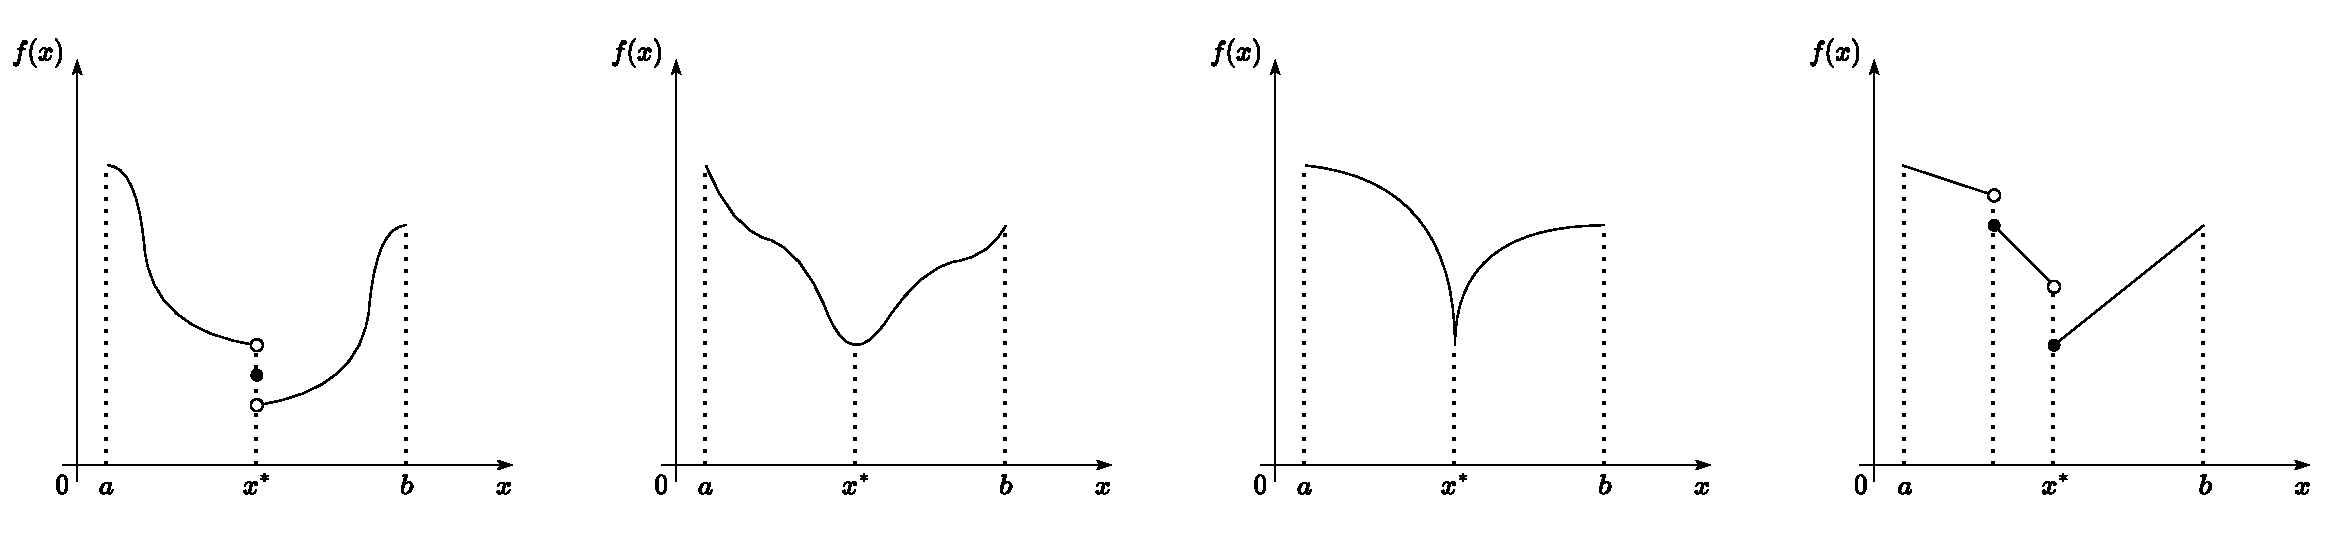
\includegraphics[keepaspectratio]{unimodal.pdf}}

}

\caption{Примеры унимодальных функций}

\end{figure}%

\subsection{Ключевое свойство унимодальных
функций}\label{ux43aux43bux44eux447ux435ux432ux43eux435-ux441ux432ux43eux439ux441ux442ux432ux43e-ux443ux43dux438ux43cux43eux434ux430ux43bux44cux43dux44bux445-ux444ux443ux43dux43aux446ux438ux439}

Пусть \(f(x)\) является унимодальной функцией на отрезке \([a, b]\).
Тогда если \(x_1 < x_2 \in [a, b]\), то:

\begin{itemize}
\tightlist
\item
  if \(f(x_1) \leq f(x_2) \to x_* \in [a, x_2]\)
\item
  if \(f(x_1) \geq f(x_2) \to x_* \in [x_1, b]\)
\end{itemize}

\textbf{Доказательство} Докажем первое утверждение. Предположим, что
\(f(x_1) \leq f(x_2)\), но \(x^* > x_2\). Тогда, поскольку
\(x_1 < x_2 < x^*\), из определения унимодальности функции \(f(x)\)
следует, что должно выполняться неравенство \(f(x_1) > f(x_2)\). Мы
получили противоречие.

\centering

\includegraphics[width=0.35\linewidth,height=\textheight,keepaspectratio]{"Unimodal lemm1.pdf"}

\includegraphics[width=0.35\linewidth,height=\textheight,keepaspectratio]{"Unimodal lemm2.pdf"}

\includegraphics[width=0.35\linewidth,height=\textheight,keepaspectratio]{"Unimodal lemm3.pdf"}

\subsection{Метод
дихотомии}\label{ux43cux435ux442ux43eux434-ux434ux438ux445ux43eux442ux43eux43cux438ux438}

Мы хотим решить следующую задачу:

\[
f(x) \to \min_{x \in [a,b]}
\]

Делим отрезок на две равные части и выбираем, основываясь на ключевом
свойстве, описанном выше, ту, которая содержит решение задачи. Наша цель
после одной итерации метода - локализовать решение в отрезке в два раза
меньшей длины.

\begin{figure}[H]

{\centering 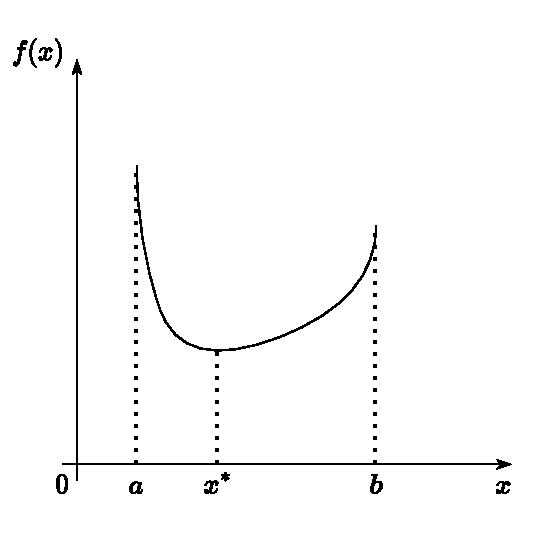
\includegraphics[width=0.4\linewidth,height=\textheight,keepaspectratio]{Dichotomy1.pdf}

}

\caption{Метод дихотомии для унимодальной функции}

\end{figure}%

Мы измеряем значение функции в середине отрезка

\begin{figure}[H]

{\centering 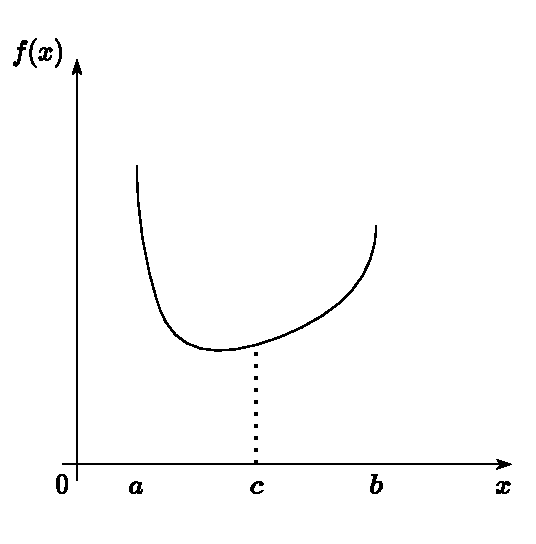
\includegraphics[width=0.4\linewidth,height=\textheight,keepaspectratio]{Dichotomy2.pdf}

}

\caption{Метод дихотомии для унимодальной функции}

\end{figure}%

Чтобы применить ключевое свойство, мы выполняем еще одно измерение.

\begin{figure}[H]

{\centering 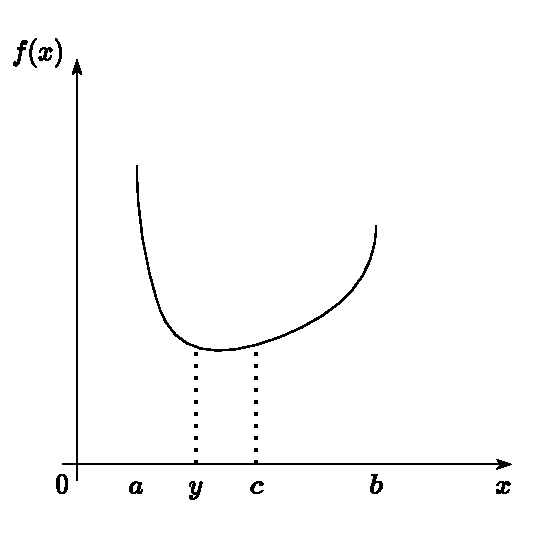
\includegraphics[width=0.4\linewidth,height=\textheight,keepaspectratio]{Dichotomy3.pdf}

}

\caption{Метод дихотомии для унимодальной функции}

\end{figure}%

Выбираем целевой отрезок. В этом случае нас все устраивает, потому что
уже разделили решение на две равные части. Но это не всегда так.

\begin{figure}[H]

{\centering 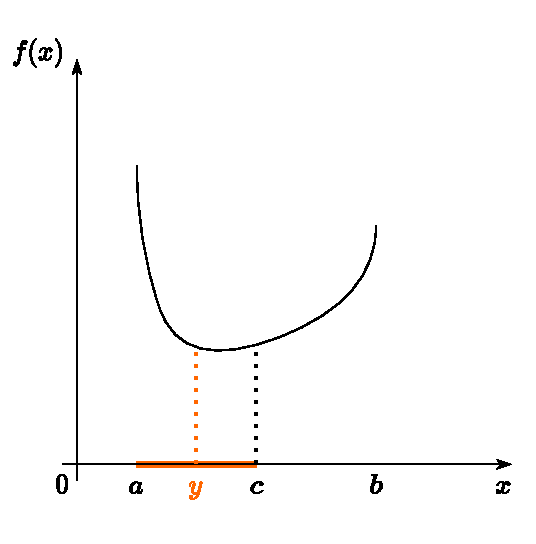
\includegraphics[width=0.4\linewidth,height=\textheight,keepaspectratio]{Dichotomy4.pdf}

}

\caption{Метод дихотомии для унимодальной функции}

\end{figure}%

Рассмотрим другую унимодальную функцию.

\begin{figure}[H]

{\centering 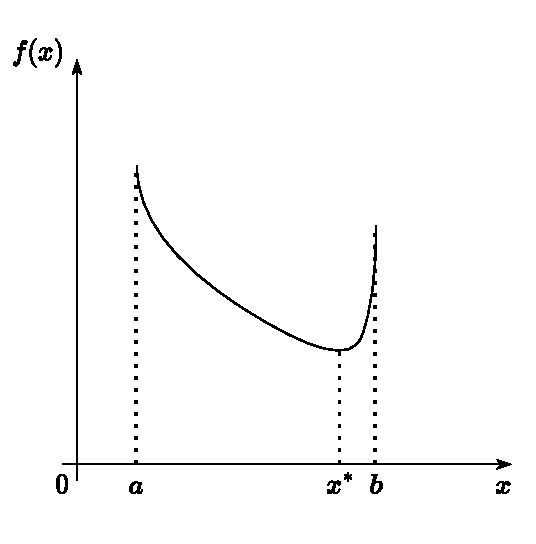
\includegraphics[width=0.4\linewidth,height=\textheight,keepaspectratio]{Dichotomy5.pdf}

}

\caption{Метод дихотомии для унимодальной функции}

\end{figure}%

Измеряем значение функции в середине отрезка.

\begin{figure}[H]

{\centering 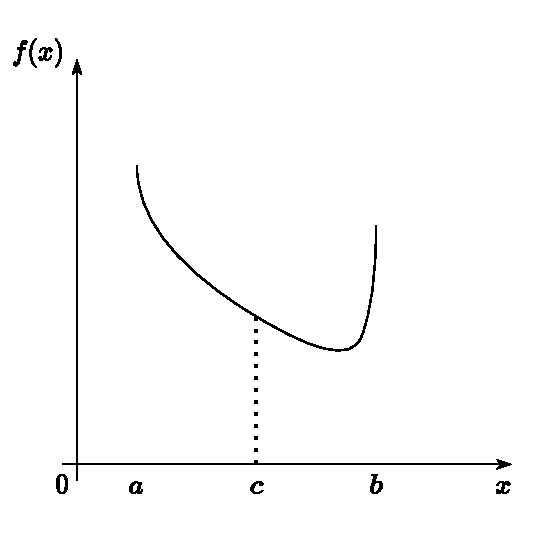
\includegraphics[width=0.4\linewidth,height=\textheight,keepaspectratio]{Dichotomy6.pdf}

}

\caption{Метод дихотомии для унимодальной функции}

\end{figure}%

Делаем еще одно измерение.

\begin{figure}[H]

{\centering 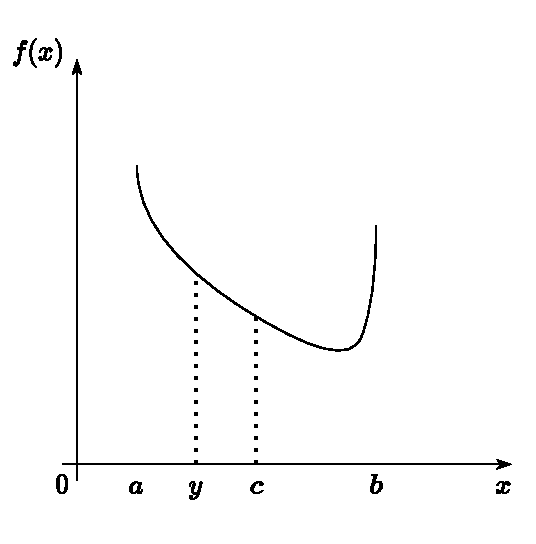
\includegraphics[width=0.4\linewidth,height=\textheight,keepaspectratio]{Dichotomy7.pdf}

}

\caption{Метод дихотомии для унимодальной функции}

\end{figure}%

Выбираем целевой отрезок. Мы можем видеть, что полученный отрезок не
является половиной исходного. Он равен \(\frac{3}{4} (b-a)\). Чтобы
исправить это, нам нужен еще один шаг алгоритма.

\begin{figure}[H]

{\centering 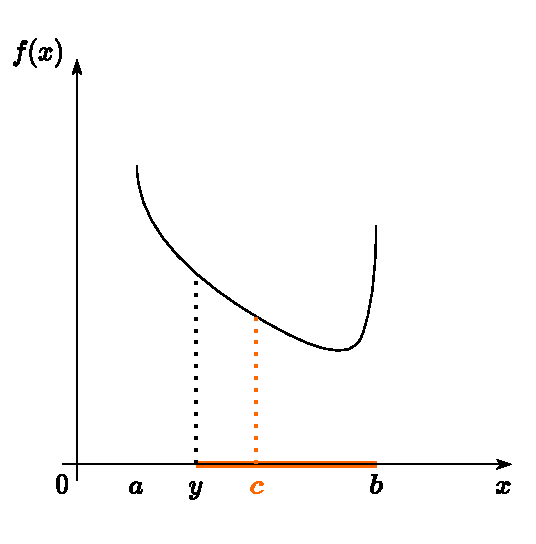
\includegraphics[width=0.4\linewidth,height=\textheight,keepaspectratio]{Dichotomy8.pdf}

}

\caption{Метод дихотомии для унимодальной функции}

\end{figure}%

После еще одного дополнительного измерения мы точно получим
\(\frac{2}{3} \frac{3}{4}(b-a) = \frac{1}{2}(b-a)\)

\begin{figure}[H]

{\centering 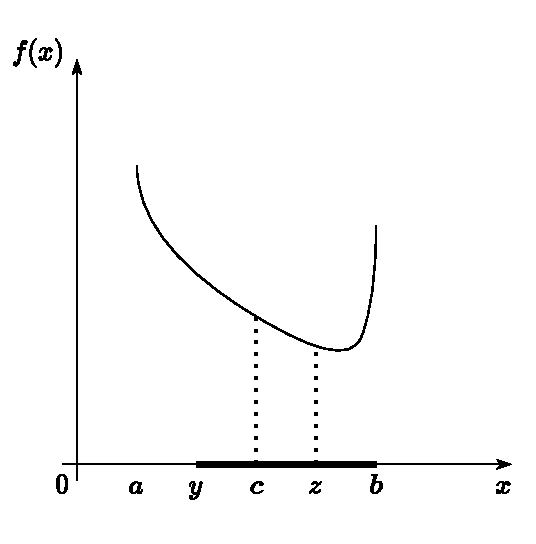
\includegraphics[width=0.4\linewidth,height=\textheight,keepaspectratio]{Dichotomy9.pdf}

}

\caption{Метод дихотомии для унимодальной функции}

\end{figure}%

В итоге, каждая последующая итерация будет требовать не более двух
измерений значений функции.

\begin{figure}[H]

{\centering 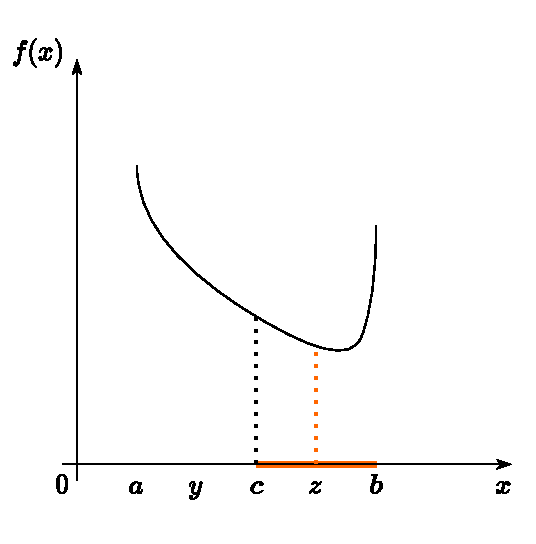
\includegraphics[width=0.4\linewidth,height=\textheight,keepaspectratio]{Dichotomy10.pdf}

}

\caption{Метод дихотомии для унимодальной функции}

\end{figure}%

\subsection{Метод дихотомии.
Алгоритм}\label{ux43cux435ux442ux43eux434-ux434ux438ux445ux43eux442ux43eux43cux438ux438.-ux430ux43bux433ux43eux440ux438ux442ux43c}

\begin{Shaded}
\begin{Highlighting}[]
\KeywordTok{def}\NormalTok{ binary\_search(f, a, b, epsilon):}
\NormalTok{   c }\OperatorTok{=}\NormalTok{ (a }\OperatorTok{+}\NormalTok{ b) }\OperatorTok{/} \DecValTok{2}
      \ControlFlowTok{while} \BuiltInTok{abs}\NormalTok{(b }\OperatorTok{{-}}\NormalTok{ a) }\OperatorTok{\textgreater{}}\NormalTok{ epsilon:}
\NormalTok{         y }\OperatorTok{=}\NormalTok{ (a }\OperatorTok{+}\NormalTok{ c) }\OperatorTok{/} \FloatTok{2.0}
         \ControlFlowTok{if}\NormalTok{ f(y) }\OperatorTok{\textless{}=}\NormalTok{ f(c):}
\NormalTok{            b }\OperatorTok{=}\NormalTok{ c}
\NormalTok{            c }\OperatorTok{=}\NormalTok{ y}
         \ControlFlowTok{else}\NormalTok{:}
\NormalTok{            z }\OperatorTok{=}\NormalTok{ (b }\OperatorTok{+}\NormalTok{ c) }\OperatorTok{/} \FloatTok{2.0}
         \ControlFlowTok{if}\NormalTok{ f(c) }\OperatorTok{\textless{}=}\NormalTok{ f(z):}
\NormalTok{            a }\OperatorTok{=}\NormalTok{ y}
\NormalTok{            b }\OperatorTok{=}\NormalTok{ z}
         \ControlFlowTok{else}\NormalTok{:}
\NormalTok{            a }\OperatorTok{=}\NormalTok{ c}
\NormalTok{            c }\OperatorTok{=}\NormalTok{ z}
      \ControlFlowTok{return}\NormalTok{ c}
\end{Highlighting}
\end{Shaded}

\subsection{Метод дихотомии.
Оценка}\label{ux43cux435ux442ux43eux434-ux434ux438ux445ux43eux442ux43eux43cux438ux438.-ux43eux446ux435ux43dux43aux430}

Длина отрезка на \(k\)-й итерации:

\[
\Delta_{k} = b_{k} - a_{k} = \dfrac{1}{2^k}(b-a)
\]

Для унимодальных функций это верно, если мы выбираем середину отрезка в
качестве выхода итерации \(x_{k}\):

\[
|x_{k} - x_*| \leq \dfrac{\Delta_{k}}{2} \leq \dfrac{1}{2^{k+1}}(b-a) \leq (0.5)^{k} \cdot  \frac{b-a}{2}
\]

Заметим, что на каждой итерации мы спрашиваем оракул не более двух раз,
поэтому количество вызовов функции равно \(N = 2 \cdot k\), что
означает:

\[
|x_{k} - x_*| \leq (0.5)^{\frac{N}{2}} \cdot \frac{b-a}{2} \leq  (0.707)^{N}  \frac{b-a}{2}
\]

Помечая правую часть последнего неравенства за \(\varepsilon\), мы
получаем количество итераций метода, необходимое для достижения точности
\(\varepsilon\):

\[
K = \left\lceil \log_2 \dfrac{b-a}{\varepsilon} - 1 \right\rceil
\]

\subsection{Метод золотого
сечения}\label{ux43cux435ux442ux43eux434-ux437ux43eux43bux43eux442ux43eux433ux43e-ux441ux435ux447ux435ux43dux438ux44f}

Идея очень похожа на метод дихотомии. На отрезке есть две точки - левая
и правая точки золотого сечения и интуитивно понятно, что на следующей
итерации одна из точек останется точкой золотого сечения.

\begin{figure}[H]

{\centering \pandocbounded{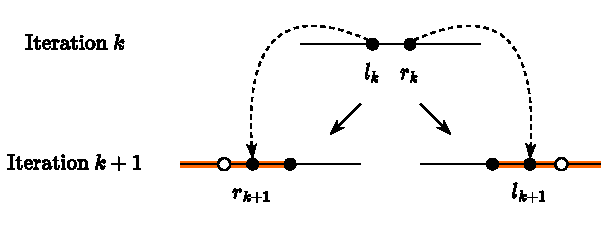
\includegraphics[keepaspectratio]{golden_search.pdf}}

}

\caption{Идея, позволяющая уменьшить количество вызовов функции}

\end{figure}%

\subsection{Метод золотого сечения.
Алгоритм}\label{ux43cux435ux442ux43eux434-ux437ux43eux43bux43eux442ux43eux433ux43e-ux441ux435ux447ux435ux43dux438ux44f.-ux430ux43bux433ux43eux440ux438ux442ux43c}

\begin{Shaded}
\begin{Highlighting}[]
\KeywordTok{def}\NormalTok{ golden\_search(f, a, b, epsilon):}
\NormalTok{   tau }\OperatorTok{=}\NormalTok{ (sqrt(}\DecValTok{5}\NormalTok{) }\OperatorTok{+} \DecValTok{1}\NormalTok{) }\OperatorTok{/} \DecValTok{2}
\NormalTok{   y }\OperatorTok{=}\NormalTok{ a }\OperatorTok{+}\NormalTok{ (b }\OperatorTok{{-}}\NormalTok{ a) }\OperatorTok{/}\NormalTok{ tau}\OperatorTok{**}\DecValTok{2}
\NormalTok{   z }\OperatorTok{=}\NormalTok{ a }\OperatorTok{+}\NormalTok{ (b }\OperatorTok{{-}}\NormalTok{ a) }\OperatorTok{/}\NormalTok{ tau}
   \ControlFlowTok{while}\NormalTok{ b }\OperatorTok{{-}}\NormalTok{ a }\OperatorTok{\textgreater{}}\NormalTok{ epsilon:}
      \ControlFlowTok{if}\NormalTok{ f(y) }\OperatorTok{\textless{}=}\NormalTok{ f(z):}
\NormalTok{         b }\OperatorTok{=}\NormalTok{ z}
\NormalTok{         z }\OperatorTok{=}\NormalTok{ y}
\NormalTok{         y }\OperatorTok{=}\NormalTok{ a }\OperatorTok{+}\NormalTok{ (b }\OperatorTok{{-}}\NormalTok{ a) }\OperatorTok{/}\NormalTok{ tau}\OperatorTok{**}\DecValTok{2}
      \ControlFlowTok{else}\NormalTok{:}
\NormalTok{         a }\OperatorTok{=}\NormalTok{ y}
\NormalTok{         y }\OperatorTok{=}\NormalTok{ z}
\NormalTok{         z }\OperatorTok{=}\NormalTok{ a }\OperatorTok{+}\NormalTok{ (b }\OperatorTok{{-}}\NormalTok{ a) }\OperatorTok{/}\NormalTok{ tau}
   \ControlFlowTok{return}\NormalTok{ (a }\OperatorTok{+}\NormalTok{ b) }\OperatorTok{/} \DecValTok{2}
\end{Highlighting}
\end{Shaded}

\subsection{Метод золотого сечения.
Оценка}\label{ux43cux435ux442ux43eux434-ux437ux43eux43bux43eux442ux43eux433ux43e-ux441ux435ux447ux435ux43dux438ux44f.-ux43eux446ux435ux43dux43aux430}

\[
|x_{k} - x_*| \leq \frac{b_{k} - a_{k}}{2} = \left( \frac{1}{\tau} \right)^{N} \frac{b - a}{2} \approx 0.618^k\frac{b - a}{2}
\]

где \(\tau = \frac{\sqrt{5} + 1}{2}\).

\begin{itemize}
\tightlist
\item
  Знаменатель геометрической прогрессии для метода золотого сечения
  \textbf{больше}, чем для метода дихотомии: \(0.618\) больше, чем
  \(0.5\).
\item
  Количество вызовов функции \textbf{меньше} для метода золотого
  сечения, чем для метода дихотомии: \(0.707\) больше (значит
  медленнее), чем \(0.618\). Для каждой итерации метода дихотомии (кроме
  первой), функция вызывается не более двух раз, в то время как для
  метода золотого сечения, она вызывается не более одного раза за
  итерацию.
\end{itemize}

\subsection{Метод параболической
интерполяции}\label{ux43cux435ux442ux43eux434-ux43fux430ux440ux430ux431ux43eux43bux438ux447ux435ux441ux43aux43eux439-ux438ux43dux442ux435ux440ux43fux43eux43bux44fux446ux438ux438}

Три точки, не лежащие на одной прямой, однозначно определяют параболу,
проходящую через них. Идея метода --- аппроксимировать функцию такой
параболой и в качестве следующего приближения взять точку её минимума.
Предположим, у нас есть 3 точки \(x_1 < x_2 < x_3\) такие, что отрезок
\([x_1, x_3]\) содержит минимум функции \(f(x)\). Тогда мы должны решить
следующую систему уравнений:

\[
ax_i^2 + bx_i + c = f_i = f(x_i), i = 1,2,3 
\]

Заметим, что эта система линейна, мы должны решить ее относительно
\(a,b,c\). Минимум этой параболы вычисляется по формуле:

\[
u = -\dfrac{b}{2a} = x_2 - \dfrac{(x_2 - x_1)^2(f_2 - f_3) - (x_2 - x_3)^2(f_2 - f_1)}{2\left[ (x_2 - x_1)(f_2 - f_3) - (x_2 - x_3)(f_2 - f_1)\right]}
\]

Заметим, что если \(f_2 < f_1, f_2 < f_3\), то \(u\) будет лежать в
\([x_1, x_3]\)

\subsection[Метод параболической интерполяции. Алгоритм
]{\texorpdfstring{Метод параболической интерполяции. Алгоритм
\footnote{Скорость сходимости этого метода суперлинейна, но локальна,
  что означает, что мы можем получить выгоду от использования этого
  метода только вблизи некоторой окрестности оптимума.
  \href{https://people.math.sc.edu/kellerlv/Quadratic_Interpolation.pdf}{\emph{Здесь}}
  доказательство суперлинейной сходимости порядка \(1.32\).}}{Метод параболической интерполяции. Алгоритм }}\label{ux43cux435ux442ux43eux434-ux43fux430ux440ux430ux431ux43eux43bux438ux447ux435ux441ux43aux43eux439-ux438ux43dux442ux435ux440ux43fux43eux43bux44fux446ux438ux438.-ux430ux43bux433ux43eux440ux438ux442ux43c-2}

\begin{Shaded}
\begin{Highlighting}[]
\KeywordTok{def}\NormalTok{ parabola\_search(f, x1, x2, x3, epsilon):}
\NormalTok{   f1, f2, f3 }\OperatorTok{=}\NormalTok{ f(x1), f(x2), f(x3)}
   \ControlFlowTok{while}\NormalTok{ x3 }\OperatorTok{{-}}\NormalTok{ x1 }\OperatorTok{\textgreater{}}\NormalTok{ epsilon:}
\NormalTok{      u }\OperatorTok{=}\NormalTok{ x2 }\OperatorTok{{-}}\NormalTok{ ((x2 }\OperatorTok{{-}}\NormalTok{ x1)}\OperatorTok{**}\DecValTok{2}\OperatorTok{*}\NormalTok{(f2 }\OperatorTok{{-}}\NormalTok{ f3) }\OperatorTok{{-}}\NormalTok{ (x2 }\OperatorTok{{-}}\NormalTok{ x3)}\OperatorTok{**}\DecValTok{2}\OperatorTok{*}\NormalTok{(f2 }\OperatorTok{{-}}\NormalTok{ f1))}\OperatorTok{/}\NormalTok{(}\DecValTok{2}\OperatorTok{*}\NormalTok{((x2 }\OperatorTok{{-}}\NormalTok{ x1)}\OperatorTok{*}\NormalTok{(f2 }\OperatorTok{{-}}\NormalTok{ f3) }\OperatorTok{{-}}\NormalTok{ (x2 }\OperatorTok{{-}}\NormalTok{ x3)}\OperatorTok{*}\NormalTok{(f2 }\OperatorTok{{-}}\NormalTok{ f1)))}
\NormalTok{      fu }\OperatorTok{=}\NormalTok{ f(u)}

      \ControlFlowTok{if}\NormalTok{ x2 }\OperatorTok{\textless{}=}\NormalTok{ u:}
         \ControlFlowTok{if}\NormalTok{ f2 }\OperatorTok{\textless{}=}\NormalTok{ fu:}
\NormalTok{            x1, x2, x3 }\OperatorTok{=}\NormalTok{ x1, x2, u}
\NormalTok{            f1, f2, f3 }\OperatorTok{=}\NormalTok{ f1, f2, fu}
         \ControlFlowTok{else}\NormalTok{:}
\NormalTok{            x1, x2, x3 }\OperatorTok{=}\NormalTok{ x2, u, x3}
\NormalTok{            f1, f2, f3 }\OperatorTok{=}\NormalTok{ f2, fu, f3}
      \ControlFlowTok{else}\NormalTok{:}
         \ControlFlowTok{if}\NormalTok{ fu }\OperatorTok{\textless{}=}\NormalTok{ f2:}
\NormalTok{            x1, x2, x3 }\OperatorTok{=}\NormalTok{ x1, u, x2}
\NormalTok{            f1, f2, f3 }\OperatorTok{=}\NormalTok{ f1, fu, f2}
         \ControlFlowTok{else}\NormalTok{:}
\NormalTok{            x1, x2, x3 }\OperatorTok{=}\NormalTok{ u, x2, x3}
\NormalTok{            f1, f2, f3 }\OperatorTok{=}\NormalTok{ fu, f2, f3}
   \ControlFlowTok{return}\NormalTok{ (x1 }\OperatorTok{+}\NormalTok{ x3)}\OperatorTok{/}\DecValTok{2}
\end{Highlighting}
\end{Shaded}

\href{https://fmin.xyz/docs/theory/inaccurate_taylor.mp4}{\pandocbounded{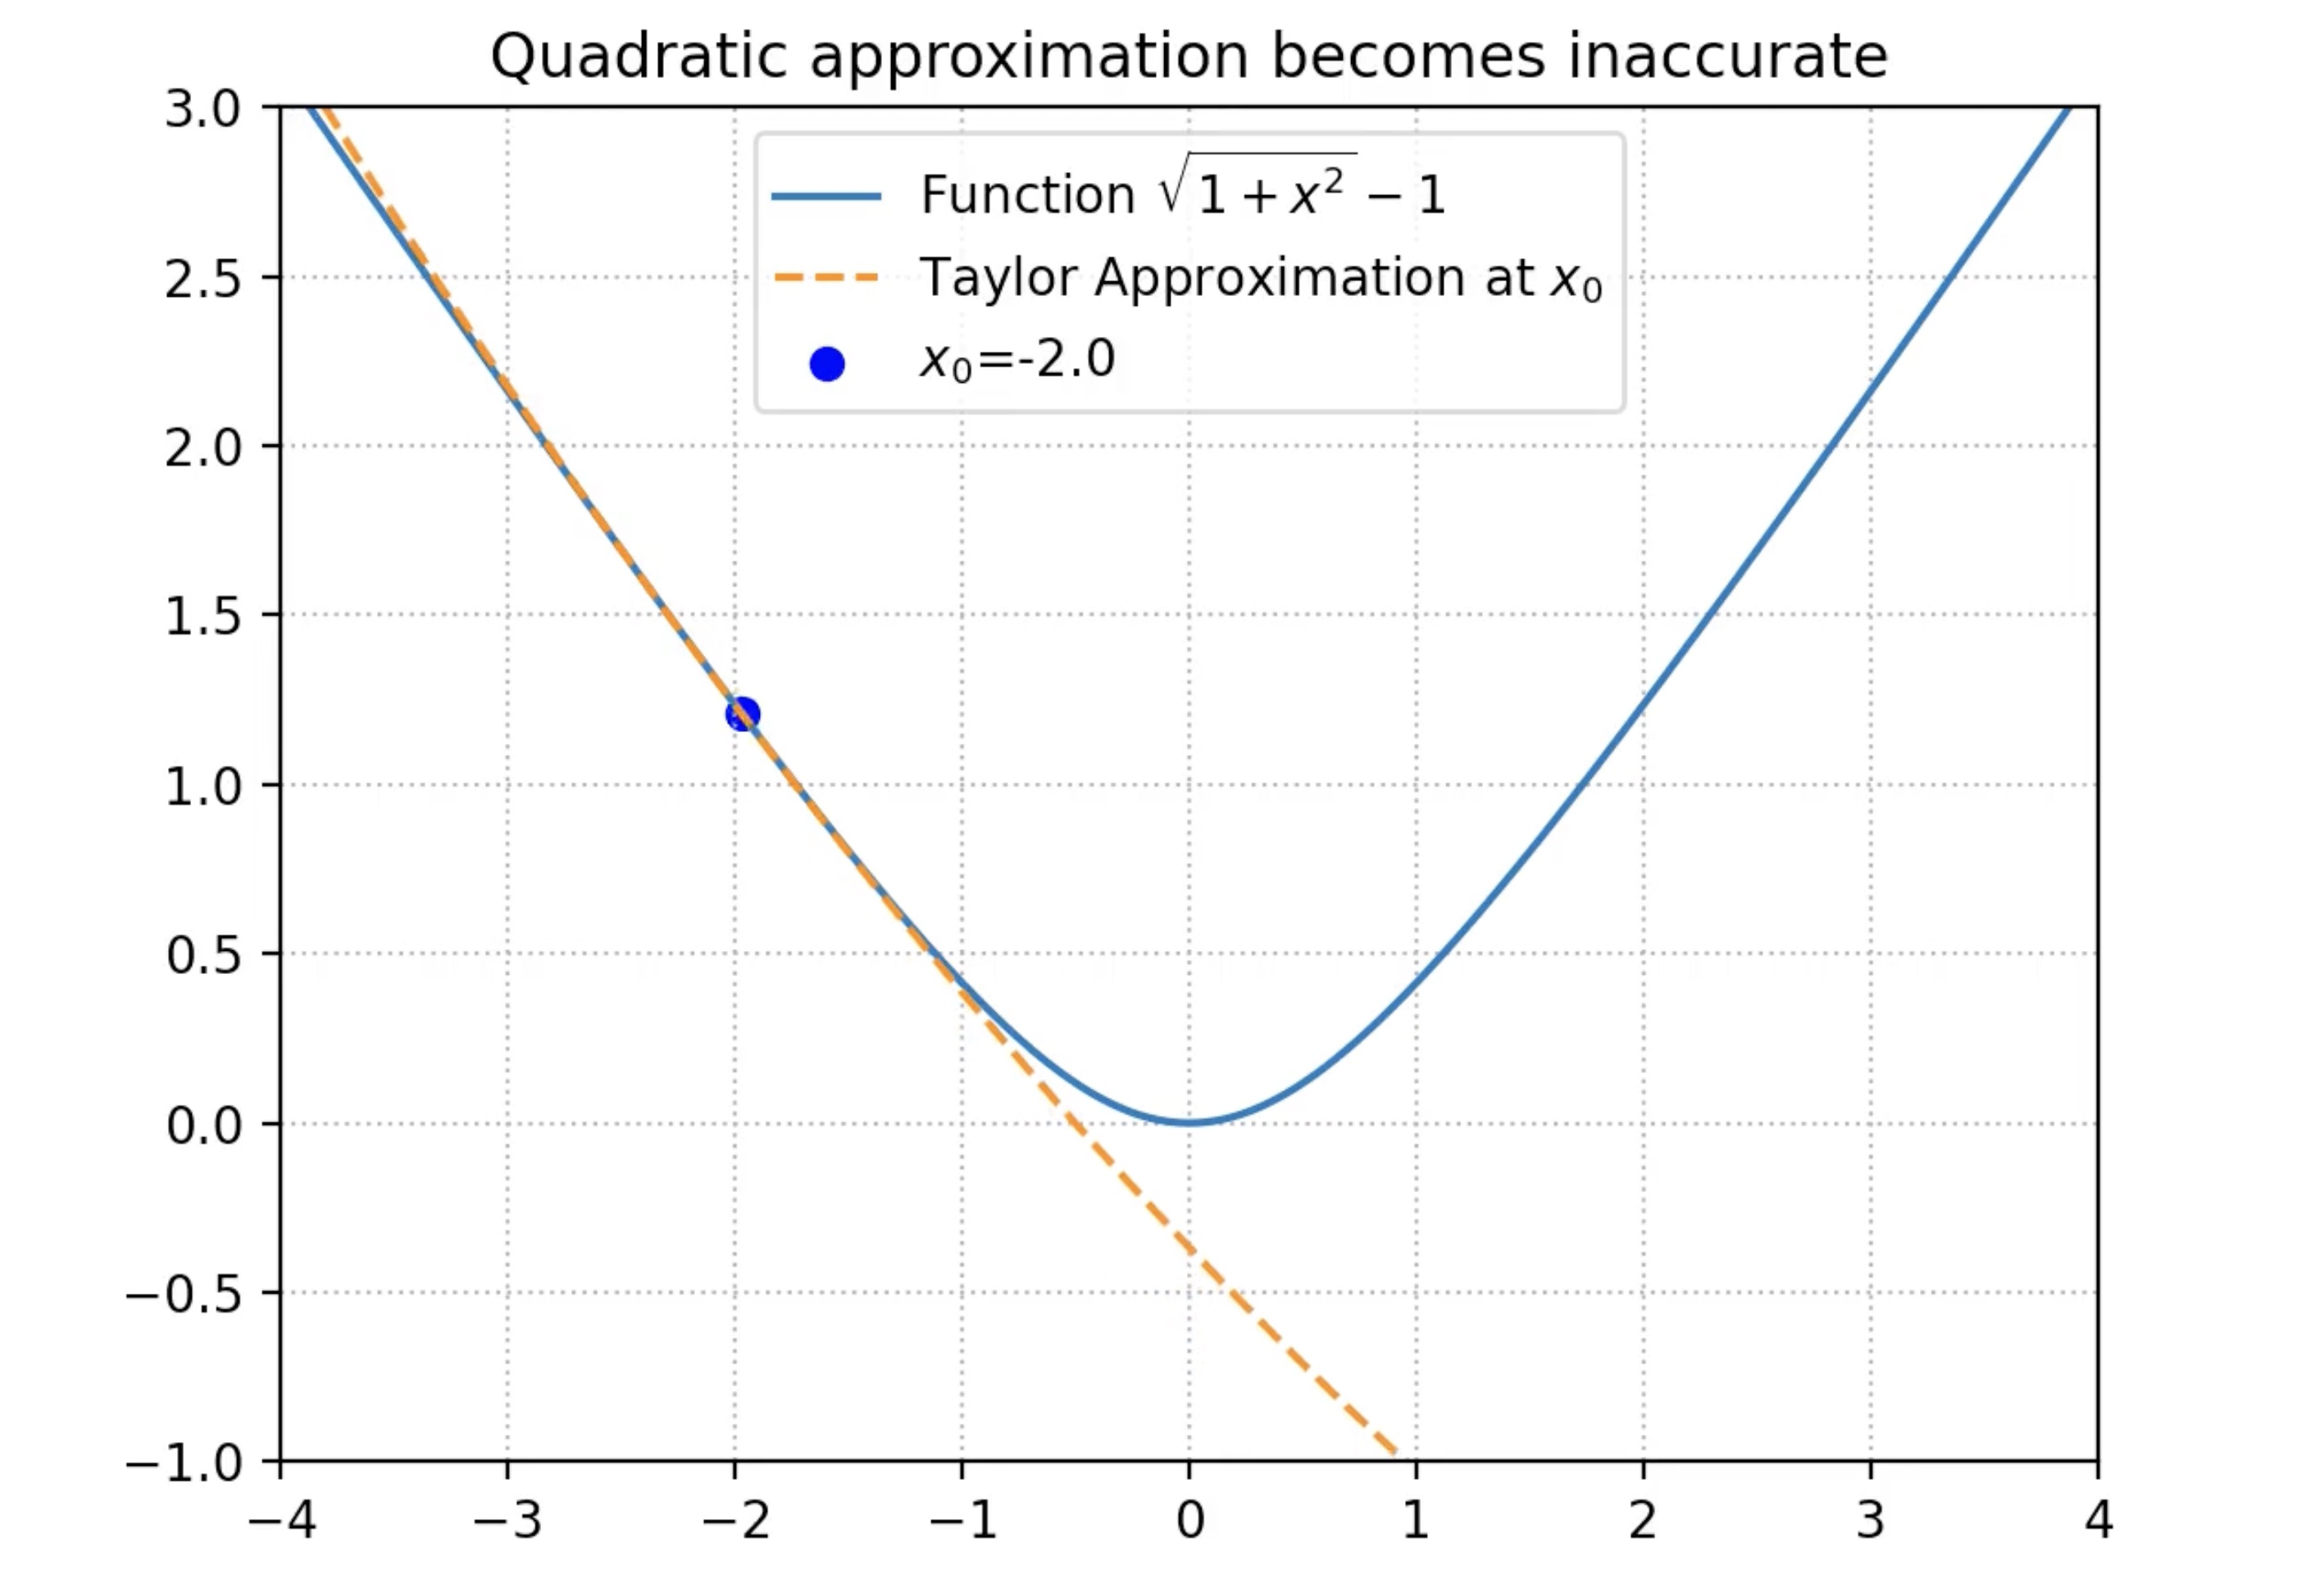
\includegraphics[keepaspectratio]{inaccurate_taylor.jpeg}}}

\subsection{Неточный линейный
поиск}\label{ux43dux435ux442ux43eux447ux43dux44bux439-ux43bux438ux43dux435ux439ux43dux44bux439-ux43fux43eux438ux441ux43a}

Нам не всегда нужно точно решать задачу минимизации. Иногда, достаточно
найти приближенное решение. Такое часто встречается в задаче выбора шага
метода оптимизации \[
\begin{split}
x_{k+1} = x_k - \alpha \nabla f(x_k) \\
\alpha = \text{argmin } f(x_{k+1}) 
\end{split}
\]

Рассмотрим скалярную функцию \(\phi(\alpha)\) в точке \(x_k\): \[
\phi(\alpha) = f(x_k - \alpha\nabla f(x_k)), \alpha \geq 0
\]

Первое приближение \(\phi(\alpha)\) в окрестности \(\alpha = 0\) равно:
\[
\phi(\alpha) \approx f(x_k) - \alpha\nabla f(x_k)^T \nabla f(x_k)
\]

\begin{figure}[H]

{\centering 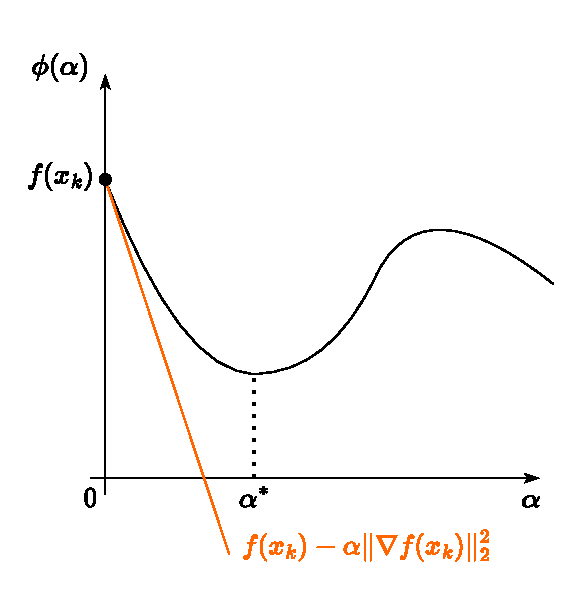
\includegraphics[width=0.5\linewidth,height=\textheight,keepaspectratio]{inexact.pdf}

}

\caption{Иллюстрация аппроксимации Тейлора \(\phi^I_0(\alpha)\)}

\end{figure}%

\subsection{Неточный линейный поиск. Условие достаточного
убывания}\label{ux43dux435ux442ux43eux447ux43dux44bux439-ux43bux438ux43dux435ux439ux43dux44bux439-ux43fux43eux438ux441ux43a.-ux443ux441ux43bux43eux432ux438ux435-ux434ux43eux441ux442ux430ux442ux43eux447ux43dux43eux433ux43e-ux443ux431ux44bux432ux430ux43dux438ux44f}

Условие неточного линейного поиска, известное как условие Армихо,
утверждает, что \(\alpha\) должно обеспечить достаточное убывание
функции \(f\), удовлетворяющее: \[
f(x_k - \alpha \nabla f (x_k)) \leq f(x_k) - c_1 \cdot \alpha\nabla f(x_k)^T \nabla f(x_k)
\]

для некоторой постоянной \(c_1 \in (0,1)\). Заметим, что установка
\(c_1 = 1\) соответствует первому приближению Тейлора \(\phi(\alpha)\).
Однако это условие может принимать очень малые значения \(\alpha\),
потенциально замедляя процесс решения. Обычно на практике используется
\(c_1 \approx 10^{-4}\).

\begin{tcolorbox}[enhanced jigsaw, title=\textcolor{quarto-callout-color}{\faInfo}\hspace{0.5em}{Example}, colframe=quarto-callout-color-frame, colbacktitle=quarto-callout-color!10!white, arc=.35mm, left=2mm, toprule=.15mm, toptitle=1mm, opacitybacktitle=0.6, bottomtitle=1mm, leftrule=.75mm, breakable, colback=white, titlerule=0mm, opacityback=0, rightrule=.15mm, bottomrule=.15mm, coltitle=black]

Если \(f(x)\) представляет собой функцию стоимости в задаче оптимизации,
важен выбор подходящего значения \(c_1\). Например, при обучении моделей
ML неправильное значение \(c_1\) может привести к очень медленной
сходимости или пропуску минимума.

\end{tcolorbox}

\begin{figure}[H]

{\centering 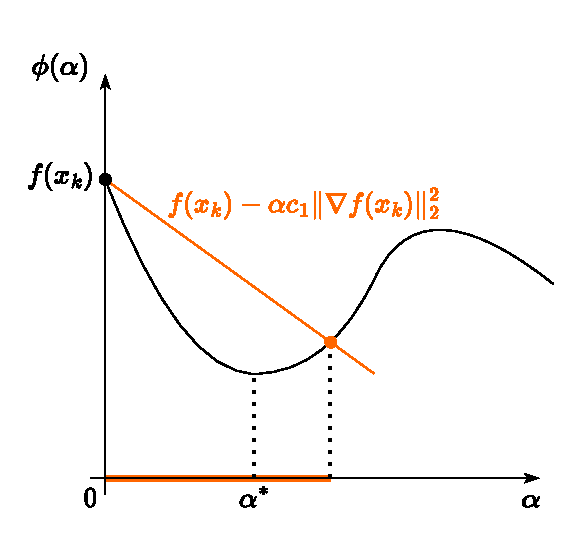
\includegraphics[width=0.5\linewidth,height=\textheight,keepaspectratio]{sufficient decrease.pdf}

}

\caption{Иллюстрация условия достаточного убывания с коэффициентом
\(c_1\)}

\end{figure}%

\subsection{Неточный линейный поиск. Условия
Гольдштейна}\label{ux43dux435ux442ux43eux447ux43dux44bux439-ux43bux438ux43dux435ux439ux43dux44bux439-ux43fux43eux438ux441ux43a.-ux443ux441ux43bux43eux432ux438ux44f-ux433ux43eux43bux44cux434ux448ux442ux435ux439ux43dux430}

Рассмотрим две линейные скалярные функции \(\phi_1(\alpha)\) и
\(\phi_2(\alpha)\): \[
\phi_1(\alpha) = f(x_k) - c_1 \alpha \|\nabla f(x_k)\|^2
\]

\[
\phi_2(\alpha) = f(x_k) - c_2 \alpha \|\nabla f(x_k)\|^2
\]

Условия Гольдштейна-Армихо находят функцию \(\phi(\alpha)\) между
\(\phi_1(\alpha)\) и \(\phi_2(\alpha)\). Обычно \(c_1 = \rho\) и
\(c_2 = 1 - \rho\), с \(\rho \in (0, 0.5)\).

\begin{figure}[H]

{\centering 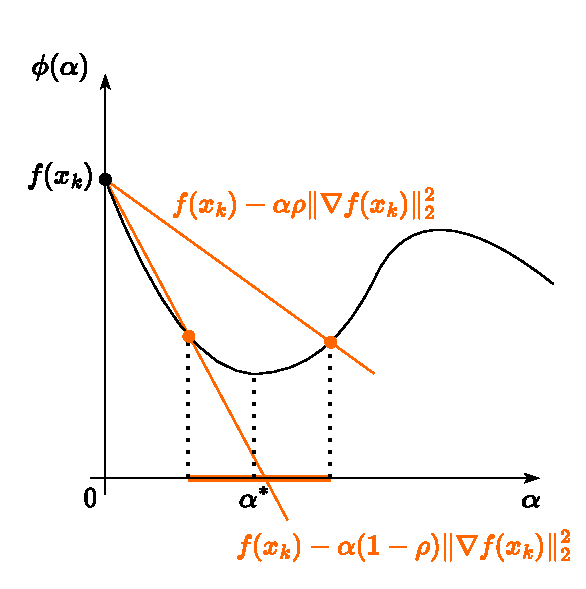
\includegraphics[width=0.5\linewidth,height=\textheight,keepaspectratio]{Goldstein.pdf}

}

\caption{Иллюстрация условий Гольдштейна}

\end{figure}%

\subsection{Неточный линейный поиск. Условие ограничения на
кривизну}\label{ux43dux435ux442ux43eux447ux43dux44bux439-ux43bux438ux43dux435ux439ux43dux44bux439-ux43fux43eux438ux441ux43a.-ux443ux441ux43bux43eux432ux438ux435-ux43eux433ux440ux430ux43dux438ux447ux435ux43dux438ux44f-ux43dux430-ux43aux440ux438ux432ux438ux437ux43dux443}

Чтобы избежать слишком коротких шагов, мы вводим второй критерий: \[
-\nabla f (x_k - \alpha \nabla f(x_k))^T \nabla f(x_k) \geq c_2 \nabla f(x_k)^T(- \nabla f(x_k))
\]

для некоторого \(c_2 \in (c_1,1)\). Здесь \(c_1\) из условия Армихо.

Левая часть является производной \(\nabla_\alpha \phi(\alpha)\),
гарантирующей, что наклон \(\phi(\alpha)\) в целевой точке не менее чем
в \(c_2\) раз больше начального наклона
\(\nabla_\alpha \phi(\alpha)(0)\).

Обычно для методов Ньютона и квазиньютоновских методов используется
\(c_2 \approx 0.9\) . В объединении условие достаточного убывания и
ограничение на кривизну образуют условия Вульфа.

\begin{figure}[H]

{\centering 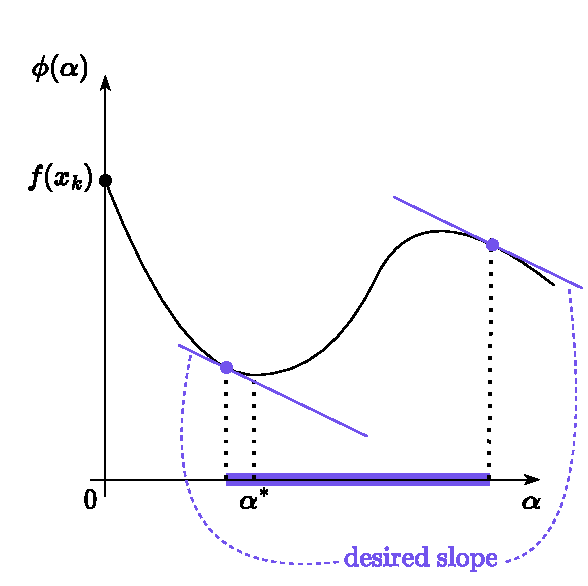
\includegraphics[width=0.35\linewidth,height=\textheight,keepaspectratio]{Curvature.pdf}

}

\caption{Иллюстрация условия ограничения на кривизну}

\end{figure}%

\subsection{Неточный линейный поиск. Условия
Вульфа}\label{ux43dux435ux442ux43eux447ux43dux44bux439-ux43bux438ux43dux435ux439ux43dux44bux439-ux43fux43eux438ux441ux43a.-ux443ux441ux43bux43eux432ux438ux44f-ux432ux443ux43bux44cux444ux430}

\[
-\nabla f (x_k - \alpha \nabla f(x_k))^T \nabla f(x_k) \geq c_2 \nabla f(x_k)^T(- \nabla f(x_k))
\]

Вместе, условие достаточного убывания и ограничение на кривизну образуют
условия Вульфа.

\begin{tcolorbox}[enhanced jigsaw, title=\textcolor{quarto-callout-color}{\faInfo}\hspace{0.5em}{Theorem}, colframe=quarto-callout-color-frame, colbacktitle=quarto-callout-color!10!white, arc=.35mm, left=2mm, toprule=.15mm, toptitle=1mm, opacitybacktitle=0.6, bottomtitle=1mm, leftrule=.75mm, breakable, colback=white, titlerule=0mm, opacityback=0, rightrule=.15mm, bottomrule=.15mm, coltitle=black]

Пусть \(f : \mathbb{R}^n \to \mathbb{R}\) непрерывно дифференцируема, и
пусть \(\phi(\alpha) = f(x_k - \alpha \nabla f(x_k))\). Предположим, что
\(\nabla f(x_k)^T p_k < 0\), где \(p_k = -\nabla f(x_k)\), делая \(p_k\)
направлением спуска. Также предположим, что \(f\) ограничена снизу вдоль
луча \(\{x_k + \alpha p_k \mid \alpha > 0\}\). Мы хотим показать, что
для \(0 < c_1 < c_2 < 1\), существуют интервалы шагов, удовлетворяющие
условиям Вульфа.

\end{tcolorbox}

\begin{figure}[H]

{\centering 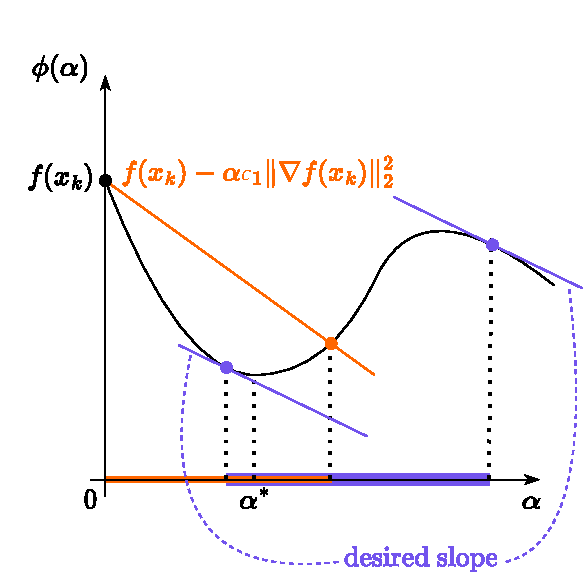
\includegraphics[width=0.4\linewidth,height=\textheight,keepaspectratio]{Wolfe.pdf}

}

\caption{Иллюстрация условий Вульфа}

\end{figure}%

\subsection{Неточный линейный поиск. Условия Вульфа.
Доказательство}\label{ux43dux435ux442ux43eux447ux43dux44bux439-ux43bux438ux43dux435ux439ux43dux44bux439-ux43fux43eux438ux441ux43a.-ux443ux441ux43bux43eux432ux438ux44f-ux432ux443ux43bux44cux444ux430.-ux434ux43eux43aux430ux437ux430ux442ux435ux43bux44cux441ux442ux432ux43e}

\begin{enumerate}
\def\labelenumi{\arabic{enumi}.}
\item
  Поскольку \(\phi(\alpha) = f(x_k + \alpha p_k)\) ограничена снизу и
  \(l(\alpha) = f(x_k) + \alpha c_1 \nabla f(x_k)^T p_k\) неограничена
  снизу (как \(\nabla f(x_k)^T p_k < 0\)), график \(l(\alpha)\) должен
  пересекать график \(\phi(\alpha)\) по крайней мере один раз. Пусть
  \(\alpha' > 0\) будет наименьшим таким значением, удовлетворяющим: \[
  f(x_k + \alpha' p_k) \leq f(x_k) + \alpha' c_1 \nabla f(x_k)^T p_k. \tag{1}
  \] Это гарантирует выполнение \textbf{условия достаточного убывания}.
\item
  По теореме о среднем значении, существует
  \(\alpha'' \in (0, \alpha')\) такое, что: \[
  f(x_k + \alpha' p_k) - f(x_k) = \alpha' \nabla f(x_k + \alpha'' p_k)^T p_k. \tag{2}
  \] Подставляя \(f(x_k + \alpha' p_k)\) из (1) в (2), мы получаем: \[
  \alpha' \nabla f(x_k + \alpha'' p_k)^T p_k \leq \alpha' c_1 \nabla f(x_k)^T p_k.
  \]
\end{enumerate}

Делим на \(\alpha' > 0\), получаем: \[
\nabla f(x_k + \alpha'' p_k)^T p_k \leq c_1 \nabla f(x_k)^T p_k. \tag{3}
\]

\begin{enumerate}
\def\labelenumi{\arabic{enumi}.}
\setcounter{enumi}{2}
\item
  Поскольку \(c_1 < c_2\) и \(\nabla f(x_k)^T p_k < 0\), неравенство
  \(c_1 \nabla f(x_k)^T p_k < c_2 \nabla f(x_k)^T p_k\) выполняется. Это
  означает, что существует \(\alpha''\) такое, что: \[
  \nabla f(x_k + \alpha'' p_k)^T p_k \leq c_2 \nabla f(x_k)^T p_k. \tag{4}
  \] Неравенства (3) и (4) вместе гарантируют выполнение условий Вульфа.
\item
  Для сильных условий Вульфа, условие ограничения на кривизну: \[
  \left| \nabla f(x_k + \alpha p_k)^T p_k \right| \leq c_2 \left| \nabla f(x_k)^T p_k \right| \tag{5}
  \] выполняется, потому что \(\nabla f(x_k + \alpha p_k)^T p_k\)
  отрицательно и ограничено снизу \(c_2 \nabla f(x_k)^T p_k\).
\item
  Из-за гладкости \(f\), существует интервал вокруг \(\alpha''\) , где
  выполняются условия Вульфа (и, следовательно, сильные условия Вульфа).
  Таким образом, доказательство завершено.
\end{enumerate}

\subsection{Бэктрекинг}\label{ux431ux44dux43aux442ux440ux435ux43aux438ux43dux433}

Бэктрекинг - это техника для нахождения шага, удовлетворяющего условию
Армихо, условиям Гольдштейна или другим критериям неточного линейного
поиска. Она начинает с относительно большого шага и итеративно уменьшает
его до тех пор, пока не будет выполнено условие.

\subsubsection{Алгоритм:}\label{ux430ux43bux433ux43eux440ux438ux442ux43c}

\begin{enumerate}
\def\labelenumi{\arabic{enumi}.}
\tightlist
\item
  Выберите начальный шаг, \(\alpha_0\), и параметры \(\beta \in (0, 1)\)
  и \(c_1 \in (0, 1)\).
\item
  Проверьте, удовлетворяет ли выбранный шаг выбранному условию
  (например, условию Армихо).
\item
  Если условие выполнено, остановитесь; в противном случае, установите
  \(\alpha := \beta \alpha\) и повторите шаг 2.
\end{enumerate}

Шаг \(\alpha\) обновляется как

\[
\alpha_{k+1} := \beta \alpha_k
\]

в каждой итерации до тех пор, пока выбранное условие не будет выполнено.

\begin{tcolorbox}[enhanced jigsaw, title=\textcolor{quarto-callout-color}{\faInfo}\hspace{0.5em}{Example}, colframe=quarto-callout-color-frame, colbacktitle=quarto-callout-color!10!white, arc=.35mm, left=2mm, toprule=.15mm, toptitle=1mm, opacitybacktitle=0.6, bottomtitle=1mm, leftrule=.75mm, breakable, colback=white, titlerule=0mm, opacityback=0, rightrule=.15mm, bottomrule=.15mm, coltitle=black]

В обучении моделей машинного обучения линейный поиск с возвратом может
использоваться для регулировки скорости обучения. Если потеря не
уменьшается достаточно, скорость обучения уменьшается мультипликативно
до тех пор, пока не будет выполнено условие Армихо.

\end{tcolorbox}

\subsection{Численная
иллюстрация}\label{ux447ux438ux441ux43bux435ux43dux43dux430ux44f-ux438ux43bux43bux44eux441ux442ux440ux430ux446ux438ux44f}

\begin{figure}[H]

{\centering \pandocbounded{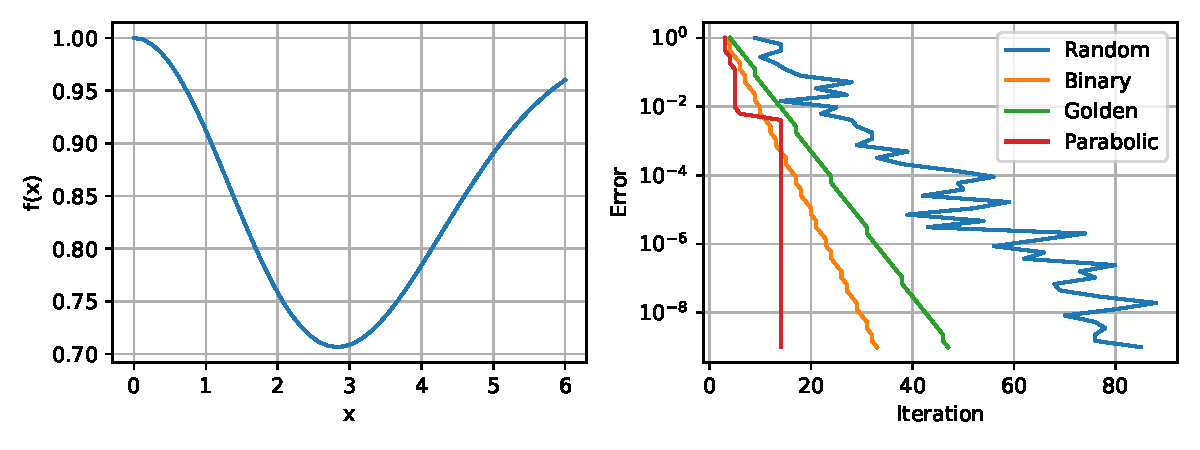
\includegraphics[keepaspectratio]{line_search_comp.pdf}}

}

\caption{Сравнение различных алгоритмов линейного поиска}

\end{figure}%

\href{https://colab.research.google.com/github/MerkulovDaniil/optim/blob/master/assets/Notebooks/Line_search.ipynb}{Открыть
в Colab \(\clubsuit\)}

\subsection{Градиентный спуск с линейным
поиском}\label{ux433ux440ux430ux434ux438ux435ux43dux442ux43dux44bux439-ux441ux43fux443ux441ux43a-ux441-ux43bux438ux43dux435ux439ux43dux44bux43c-ux43fux43eux438ux441ux43aux43eux43c}

\href{https://fmin.xyz/docs/visualizations/ls_gd.mp4}{\pandocbounded{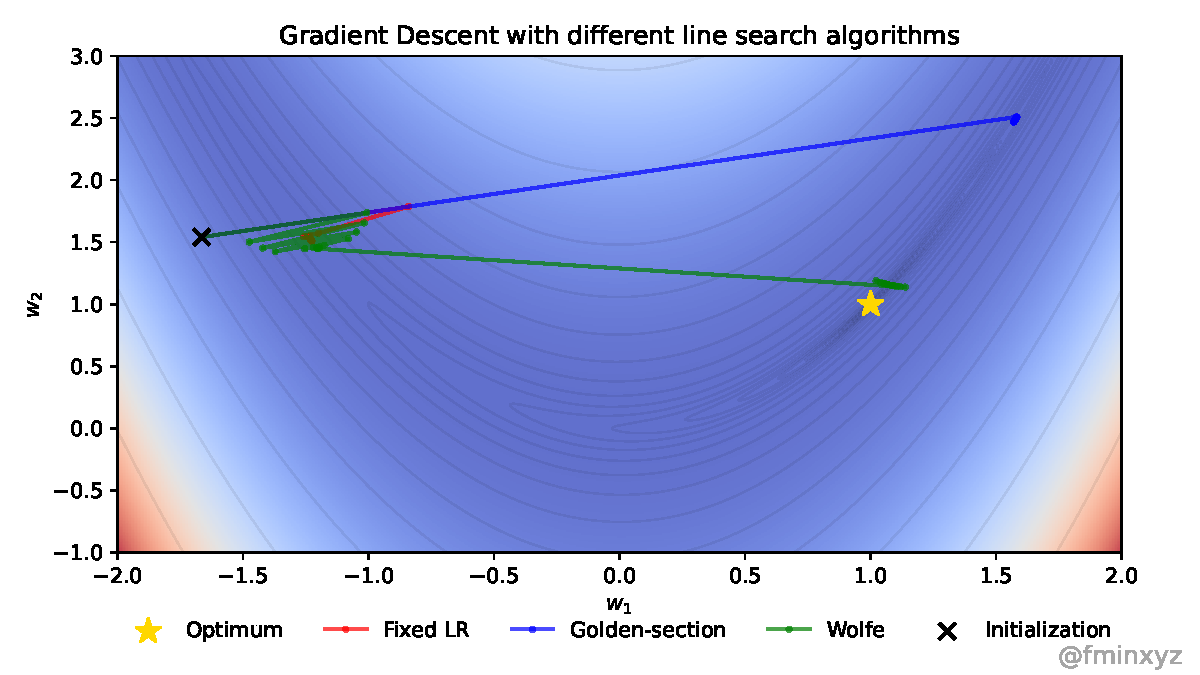
\includegraphics[keepaspectratio]{gd_ls.pdf}}}

:::

\section{Задачи}\label{ux437ux430ux434ux430ux447ux438}

\subsection{Задача 1}\label{ux437ux430ux434ux430ux447ux430-1}

\begin{tcolorbox}[enhanced jigsaw, title=\textcolor{quarto-callout-color}{\faInfo}\hspace{0.5em}{Example}, colframe=quarto-callout-color-frame, colbacktitle=quarto-callout-color!10!white, arc=.35mm, left=2mm, toprule=.15mm, toptitle=1mm, opacitybacktitle=0.6, bottomtitle=1mm, leftrule=.75mm, breakable, colback=white, titlerule=0mm, opacityback=0, rightrule=.15mm, bottomrule=.15mm, coltitle=black]

Найдите \(\nabla f(x)\), если \(f(x) = \dfrac{1}{2}x^TAx + b^Tx + c\).

\end{tcolorbox}

\subsection{Задача 2}\label{ux437ux430ux434ux430ux447ux430-2}

\begin{tcolorbox}[enhanced jigsaw, title=\textcolor{quarto-callout-color}{\faInfo}\hspace{0.5em}{Example}, colframe=quarto-callout-color-frame, colbacktitle=quarto-callout-color!10!white, arc=.35mm, left=2mm, toprule=.15mm, toptitle=1mm, opacitybacktitle=0.6, bottomtitle=1mm, leftrule=.75mm, breakable, colback=white, titlerule=0mm, opacityback=0, rightrule=.15mm, bottomrule=.15mm, coltitle=black]

Найдите \(\nabla f(X)\), если \(f(X) = tr(AX^{-1}B)\)

\end{tcolorbox}

\subsection{Задача 3}\label{ux437ux430ux434ux430ux447ux430-3}

\begin{tcolorbox}[enhanced jigsaw, title=\textcolor{quarto-callout-color}{\faInfo}\hspace{0.5em}{Example}, colframe=quarto-callout-color-frame, colbacktitle=quarto-callout-color!10!white, arc=.35mm, left=2mm, toprule=.15mm, toptitle=1mm, opacitybacktitle=0.6, bottomtitle=1mm, leftrule=.75mm, breakable, colback=white, titlerule=0mm, opacityback=0, rightrule=.15mm, bottomrule=.15mm, coltitle=black]

Найдите градиент \(\nabla f(x)\) и гессиан \(\nabla^2 f(x)\), если
\(f(x) = \frac{1}{3}\Vert x\Vert _2^3\)

\end{tcolorbox}

\section{Задачи на
дом}\label{ux437ux430ux434ux430ux447ux438-ux43dux430-ux434ux43eux43c}

\subsection{Линейный
поиск}\label{ux43bux438ux43dux435ux439ux43dux44bux439-ux43fux43eux438ux441ux43a-1}

\begin{enumerate}
\def\labelenumi{\arabic{enumi}.}
\item
  {[}10 баллов{]} Рассмотрим строго выпуклую квадратичную функцию
  \(f: \mathbb{R}^n \rightarrow \mathbb{R}\), и пусть мы начинаем из
  точки \(x_k \in \mathbb{R}^n\) двигаться в направлении антиградиента
  \(-\nabla f(x_k)\), при этом \(\nabla f(x_k)\neq 0\). Покажите, что
  минимум \(f\) вдоль этого направления как функция шага \(\alpha\), для
  убывающей функции в точке \(x_k\), удовлетворяет условию Армихо для
  любого \(c_1\) в диапазоне \(0 \leq c_1 \leq \frac{1}{2}\). В
  частности, покажите, что следующее неравенство выполняется в
  оптимальном \(\alpha^*\): \[
   \varphi(\alpha) = f(x_{k+1}) = f(x_k - \alpha \nabla f(x_k)) \leq f(x_k) - c_1 \alpha \|\nabla f(x_k)\|_2^2
   \]
\item
  \textbf{Реализация и тестирование условий линейного поиска в
  градиентном спуске} {[}36 баллов{]} \[
   x_{k+1} = x_k - \alpha \nabla f(x_k)
   \] В этом задании мы будем модифицировать существующий Python код для
  градиентного спуска, чтобы включить различные условия линейного
  поиска. Мы протестируем эти модификации на двух функциях: квадратичной
  функции и функции Розенброка. Основные цели - понять, как различные
  стратегии линейного поиска влияют на сходимость алгоритма градиентного
  спуска и сравнить их эффективность на основе количества вызовов
  функции.

\begin{Shaded}
\begin{Highlighting}[]
\ImportTok{import}\NormalTok{ numpy }\ImportTok{as}\NormalTok{ np}
\ImportTok{import}\NormalTok{ matplotlib.pyplot }\ImportTok{as}\NormalTok{ plt}
\ImportTok{from}\NormalTok{ scipy.optimize }\ImportTok{import}\NormalTok{ minimize\_scalar}
\NormalTok{np.random.seed(}\DecValTok{214}\NormalTok{)}

\CommentTok{\# Define the quadratic function and its gradient}
\KeywordTok{def}\NormalTok{ quadratic\_function(x, A, b):}
    \ControlFlowTok{return} \FloatTok{0.5} \OperatorTok{*}\NormalTok{ np.dot(x.T, np.dot(A, x)) }\OperatorTok{{-}}\NormalTok{ np.dot(b.T, x)}

\KeywordTok{def}\NormalTok{ grad\_quadratic(x, A, b):}
    \ControlFlowTok{return}\NormalTok{ np.dot(A, x) }\OperatorTok{{-}}\NormalTok{ b}

\CommentTok{\# Generate a 2D quadratic problem with a specified condition number}
\KeywordTok{def}\NormalTok{ generate\_quadratic\_problem(cond\_number):}
    \CommentTok{\# Random symmetric matrix}
\NormalTok{    M }\OperatorTok{=}\NormalTok{ np.random.randn(}\DecValTok{2}\NormalTok{, }\DecValTok{2}\NormalTok{)}
\NormalTok{    M }\OperatorTok{=}\NormalTok{ np.dot(M, M.T)}

    \CommentTok{\# Ensure the matrix has the desired condition number}
\NormalTok{    U, s, V }\OperatorTok{=}\NormalTok{ np.linalg.svd(M)}
\NormalTok{    s }\OperatorTok{=}\NormalTok{ np.linspace(cond\_number, }\DecValTok{1}\NormalTok{, }\BuiltInTok{len}\NormalTok{(s))  }\CommentTok{\# Spread the singular values}
\NormalTok{    A }\OperatorTok{=}\NormalTok{ np.dot(U, np.dot(np.diag(s), V))}

    \CommentTok{\# Random b}
\NormalTok{    b }\OperatorTok{=}\NormalTok{ np.random.randn(}\DecValTok{2}\NormalTok{)}

    \ControlFlowTok{return}\NormalTok{ A, b}

\CommentTok{\# Gradient descent function}
\KeywordTok{def}\NormalTok{ gradient\_descent(start\_point, A, b, stepsize\_func, max\_iter}\OperatorTok{=}\DecValTok{100}\NormalTok{):}
\NormalTok{    x }\OperatorTok{=}\NormalTok{ start\_point.copy()}
\NormalTok{    trajectory }\OperatorTok{=}\NormalTok{ [x.copy()]}

    \ControlFlowTok{for}\NormalTok{ i }\KeywordTok{in} \BuiltInTok{range}\NormalTok{(max\_iter):}
\NormalTok{        grad }\OperatorTok{=}\NormalTok{ grad\_quadratic(x, A, b)}
\NormalTok{        step\_size }\OperatorTok{=}\NormalTok{ stepsize\_func(x, grad)}
\NormalTok{        x }\OperatorTok{{-}=}\NormalTok{ step\_size }\OperatorTok{*}\NormalTok{ grad}
\NormalTok{        trajectory.append(x.copy())}

    \ControlFlowTok{return}\NormalTok{ np.array(trajectory)}

\CommentTok{\# Backtracking line search strategy using scipy}
\KeywordTok{def}\NormalTok{ backtracking\_line\_search(x, grad, A, b, alpha}\OperatorTok{=}\FloatTok{0.3}\NormalTok{, beta}\OperatorTok{=}\FloatTok{0.8}\NormalTok{):}
    \KeywordTok{def}\NormalTok{ objective(t):}
        \ControlFlowTok{return}\NormalTok{ quadratic\_function(x }\OperatorTok{{-}}\NormalTok{ t }\OperatorTok{*}\NormalTok{ grad, A, b)}
\NormalTok{    res }\OperatorTok{=}\NormalTok{ minimize\_scalar(objective, method}\OperatorTok{=}\StringTok{\textquotesingle{}golden\textquotesingle{}}\NormalTok{)}
    \ControlFlowTok{return}\NormalTok{ res.x}

\CommentTok{\# Generate ill{-}posed problem}
\NormalTok{cond\_number }\OperatorTok{=} \DecValTok{30}
\NormalTok{A, b }\OperatorTok{=}\NormalTok{ generate\_quadratic\_problem(cond\_number)}

\CommentTok{\# Starting point}
\NormalTok{start\_point }\OperatorTok{=}\NormalTok{ np.array([}\FloatTok{1.0}\NormalTok{, }\FloatTok{1.8}\NormalTok{])}

\CommentTok{\# Perform gradient descent with both strategies}
\NormalTok{trajectory\_fixed }\OperatorTok{=}\NormalTok{ gradient\_descent(start\_point, A, b, }\KeywordTok{lambda}\NormalTok{ x, g: }\FloatTok{5e{-}2}\NormalTok{)}
\NormalTok{trajectory\_backtracking }\OperatorTok{=}\NormalTok{ gradient\_descent(start\_point, A, b, }\KeywordTok{lambda}\NormalTok{ x, g: backtracking\_line\_search(x, g, A, b))}

\CommentTok{\# Plot the trajectories on a contour plot}
\NormalTok{x1, x2 }\OperatorTok{=}\NormalTok{ np.meshgrid(np.linspace(}\OperatorTok{{-}}\DecValTok{2}\NormalTok{, }\DecValTok{2}\NormalTok{, }\DecValTok{400}\NormalTok{), np.linspace(}\OperatorTok{{-}}\DecValTok{2}\NormalTok{, }\DecValTok{2}\NormalTok{, }\DecValTok{400}\NormalTok{))}
\NormalTok{Z }\OperatorTok{=}\NormalTok{ np.array([quadratic\_function(np.array([x, y]), A, b) }\ControlFlowTok{for}\NormalTok{ x, y }\KeywordTok{in} \BuiltInTok{zip}\NormalTok{(x1.flatten(), x2.flatten())]).reshape(x1.shape)}

\NormalTok{plt.figure(figsize}\OperatorTok{=}\NormalTok{(}\DecValTok{10}\NormalTok{, }\DecValTok{8}\NormalTok{))}
\NormalTok{plt.contour(x1, x2, Z, levels}\OperatorTok{=}\DecValTok{50}\NormalTok{, cmap}\OperatorTok{=}\StringTok{\textquotesingle{}viridis\textquotesingle{}}\NormalTok{)}
\NormalTok{plt.plot(trajectory\_fixed[:, }\DecValTok{0}\NormalTok{], trajectory\_fixed[:, }\DecValTok{1}\NormalTok{], }\StringTok{\textquotesingle{}o{-}\textquotesingle{}}\NormalTok{, label}\OperatorTok{=}\StringTok{\textquotesingle{}Fixed Step Size\textquotesingle{}}\NormalTok{)}
\NormalTok{plt.plot(trajectory\_backtracking[:, }\DecValTok{0}\NormalTok{], trajectory\_backtracking[:, }\DecValTok{1}\NormalTok{], }\StringTok{\textquotesingle{}o{-}\textquotesingle{}}\NormalTok{, label}\OperatorTok{=}\StringTok{\textquotesingle{}Backtracking Line Search\textquotesingle{}}\NormalTok{)}

\CommentTok{\# Add markers for start and optimal points}
\NormalTok{plt.plot(start\_point[}\DecValTok{0}\NormalTok{], start\_point[}\DecValTok{1}\NormalTok{], }\StringTok{\textquotesingle{}ro\textquotesingle{}}\NormalTok{, label}\OperatorTok{=}\StringTok{\textquotesingle{}Start Point\textquotesingle{}}\NormalTok{)}
\NormalTok{optimal\_point }\OperatorTok{=}\NormalTok{ np.linalg.solve(A, b)}
\NormalTok{plt.plot(optimal\_point[}\DecValTok{0}\NormalTok{], optimal\_point[}\DecValTok{1}\NormalTok{], }\StringTok{\textquotesingle{}y*\textquotesingle{}}\NormalTok{, markersize}\OperatorTok{=}\DecValTok{15}\NormalTok{, label}\OperatorTok{=}\StringTok{\textquotesingle{}Optimal Point\textquotesingle{}}\NormalTok{)}

\NormalTok{plt.legend()}
\NormalTok{plt.title(}\StringTok{\textquotesingle{}Gradient Descent Trajectories on Quadratic Function\textquotesingle{}}\NormalTok{)}
\NormalTok{plt.xlabel(}\StringTok{\textquotesingle{}x1\textquotesingle{}}\NormalTok{)}
\NormalTok{plt.ylabel(}\StringTok{\textquotesingle{}x2\textquotesingle{}}\NormalTok{)}
\NormalTok{plt.savefig(}\StringTok{"linesearch.svg"}\NormalTok{)}
\NormalTok{plt.show()}
\end{Highlighting}
\end{Shaded}

  Начните с ознакомления с предоставленным Python кодом. Этот код
  реализует градиентный спуск с фиксированным шагом и бэктрекингом на
  квадратичной функции. Ознакомьтесь с тем, как реализованы функции
  градиентного спуска и стратегии размера шага.

  \begin{enumerate}
  \def\labelenumii{\arabic{enumii}.}
  \item
    {[}10/36 баллов{]} Измените функцию градиентного спуска, чтобы
    включить следующие условия линейного поиска:

    \begin{enumerate}
    \def\labelenumiii{\arabic{enumiii}.}
    \tightlist
    \item
      Дихотомия
    \item
      Условие достаточного убывания
    \item
      Условия Вольфа
    \item
      Шаг Поляка \[
       \alpha_k = \frac{f(x_k) - f^*}{\|\nabla f(x_k)\|_2^2},
       \] где \(f^*\) - оптимальное значение функции. Кажется странным
      использовать оптимальное значение функции в размере шага, но есть
      варианты оценить его даже без знания оптимального значения.\\
    \item
      Метод знака градиента: \[
       \alpha_k = \frac{1}{\|\nabla f(x_k)\|_2},
       \] Протестируйте модифицированный алгоритм градиентного спуска с
      реализованными стратегиями поиска размера шага на предоставленной
      квадратичной функции. Постройте траектории по итерациям для
      каждого условия. Выберите и укажите гиперпараметры для неточных
      условий линейного поиска. Выберите и укажите \textbf{критерий
      остановки}. Начните с точки \(x_0 = (-1, 2)^T\).
    \end{enumerate}
  \item
    {[}8/36 баллов{]} Сравните эти 7 методов с точки зрения бюджета.
    Постройте график значения функции от количества вызовов функции для
    каждого метода на одном графике.
  \item
    {[}10/36 баллов{]} Постройте траекторию для другой функции с тем же
    набором методов \[
     f(x_1, x_2) =  10(x_2 − x_1^2)^2 + (x_1 − 1)^2
     \] с \(x_0 = (-1, 2)^T\). Возможно, вам придется подстроить
    гиперпараметры.
  \item
    {[}8/36 баллов{]} Постройте тот же график значения функции от
    количества вызовов функции для этого эксперимента.
  \end{enumerate}
\end{enumerate}

\subsection{Матрично-векторное
дифференцирование}\label{ux43cux430ux442ux440ux438ux447ux43dux43e-ux432ux435ux43aux442ux43eux440ux43dux43eux435-ux434ux438ux444ux444ux435ux440ux435ux43dux446ux438ux440ux43eux432ux430ux43dux438ux435-1}

\begin{enumerate}
\def\labelenumi{\arabic{enumi}.}
\item
  {[}6 баллов{]} Найдите градиент \(\nabla f(x)\) и гессиан
  \(f^{\prime\prime}(x)\), если
  \(f(x) = \frac{1}{2}\Vert A - xx^T\Vert ^2_F, A \in \mathbb{S}^n\)
\item
  {[}6 баллов{]} Найдите градиент \(\nabla f(x)\) и гессиан \(f''(x)\),
  если \(f(x) = \dfrac{1}{2} \Vert Ax - b\Vert^2_2\).
\item
  {[}8 баллов{]} Найдите градиент \(\nabla f(x)\) и гессиан \(f''(x)\),
  если \[
   f(x) = \frac1m \sum\limits_{i=1}^m \log \left( 1 + \exp(a_i^{T}x) \right) + \frac{\mu}{2}\Vert x\Vert _2^2, \; a_i, x \in \mathbb R^n, \; \mu>0
   \]
\item
  {[}8 баллов{]} Найдите градиент \(\nabla_A f(A)\) от следа функции
  матричной экспоненты \(f(A) = \text{tr}(e^A)\) с точки зрения \(A\).\\
  Подсказка: Используйте определение матричной экспоненты. Используйте
  определение дифференциала
  \(df = f(A + dA) - f(A) + o(\Vert dA \Vert)\) с пределом
  \(\Vert dA \Vert \to 0\).
\item
  {[}20 баллов{]} \textbf{Главные компоненты через вычисление
  градиента.} Пусть есть набор данных
  \(\{x_i\}_{i=1}^N, x_i \in \mathbb{R}^D\), который мы хотим
  преобразовать в набор данных меньшей размерности \(d\) с помощью
  проекции на линейное подпространство, определяемое матрицей
  \(P \in \mathbb{R}^{D \times d}\). Ортогональная проекция вектора
  \(x\) на это подпространство может быть вычислена как
  \(P(P^TP)^{-1}P^Tx\). Чтобы найти оптимальную матрицу \(P\),
  рассмотрим следующую задачу оптимизации: \[
   F(P) = \sum_{i=1}^N \|x_i - P(P^TP)^{-1}P^Tx_i\|^2 = N \cdot \text{tr}\left((I - P(P^TP)^{-1}P^T)^2 S\right) \to \min_{P \in \mathbb{R}^{D \times d}},
   \] где \(S = \frac{1}{N} \sum_{i=1}^N x_i x_i^T\) - выборочная
  ковариационная матрица для нормализованного набора данных.

  \begin{enumerate}
  \def\labelenumii{\arabic{enumii}.}
  \item
    Найдите градиент \(\nabla_P F(P)\), рассчитанный для произвольной
    матрицы \(P\) с ортогональными столбцами, т.е. \(P : P^T P = I\).

    \emph{Подсказка: При вычислении дифференциала \(dF(P)\), сначала
    рассмотрите \(P\) как произвольную матрицу, а затем используйте
    ортогональность столбцов \(P\) в полученном выражении.}
  \item
    Рассмотрите разложение матрицы \(S\) на собственные значения: \[
     S = Q \Lambda Q^T,
     \] где \(\Lambda\) - диагональная матрица с собственными значениями
    на диагонали, и
    \(Q = [q_1 | q_2 | \ldots | q_D] \in \mathbb{R}^{D \times D}\) -
    ортогональная матрица, состоящая из собственных векторов \(q_i\) в
    качестве столбцов. Докажите следующее:

    \begin{enumerate}
    \def\labelenumiii{\arabic{enumiii}.}
    \tightlist
    \item
      Градиент \(\nabla_P F(P)\) равен нулю для любой матрицы \(P\),
      состоящей из \(d\) различных собственных векторов \(q_i\) в
      качестве ее столбцов.
    \item
      Минимальное значение \(F(P)\) достигается для матрицы \(P\),
      состоящей из собственных векторов \(q_i\), соответствующих
      наибольшим собственным значениям \(S\).
    \end{enumerate}
  \end{enumerate}
\end{enumerate}




\end{document}
